\documentclass{article}
\usepackage[document]{ragged2e}
\usepackage{enumitem}
\usepackage{amssymb}
\usepackage[spaces,hyphens]{url}
\usepackage{amsthm}
\usepackage{bbm}
\usepackage{multicol}
\usepackage{dsfont}
\usepackage{fullpage}
\usepackage{listings}
\usepackage{fancyhdr}
\usepackage{titlesec}
\usepackage{hyperref}
\usepackage{xcolor}
\usepackage{stmaryrd}
\usepackage{tikzpagenodes}
\usepackage[T1]{fontenc}
\usepackage[utf8]{inputenc}
\usepackage{CJKutf8}
\usepackage[english]{babel}
\usepackage{titlesec}
\usepackage{pgfplots}
\pgfplotsset{width=10cm,compat=1.9}
\usepgfplotslibrary{external} 
\usepackage{tikz,tkz-tab,amsmath}
\usetikzlibrary{arrows}
\graphicspath{ {./images/} }
\newcommand\E{e}
\newcommand\R{\mathbb{R}}
\newcommand\N{\mathbb{N}}
\newcommand\Z{\mathbb{Z}}
\newcommand\K{\mathbb{K}}
\newcommand\Q{\mathbb{Q}}
\newcommand\C{\mathbb{C}}
\newcommand\T{\mathcal{T}}
\usepackage[headsep=1cm, headheight=1cm]{geometry}
% !TeX spellcheck = en_GB 

\newcommand\dspst{\displaystyle}
\def\prop#1{\underline{\textbf{#1}}}

\def\changemargin#1#2{\list{}{\rightmargin#2\leftmargin#1}\item[]}
\let\endchangemargin=\endlist

%\titleformat{\part}[block]{\filcenter}{}(1em){}
\titleformat{\part}[block]{\Huge\bfseries\filcenter}{\partname{} \\ \thepart}{1em}{\huge}


%Defines emphasis color
\definecolor{rycolor}{RGB}{200,20,255}
\definecolor{note}{RGB}{100,100,100}
\definecolor{background}{RGB}{0,20,70}

%Defining a multi-line comment
\newcommand{\comment}[1]{}

\title{Computational Biology Project \\ A model of sympatric speciation with two evolving traits}
%{proposed by Michael Kopp}
\author{Alice Clément, Christopher Mazzerbo}
\date{Last updated on \today}


\begin{document}

\lstset{ 
  backgroundcolor=\color{background},
  basicstyle=\footnotesize\color{white},
  breakatwhitespace=false,
  breaklines=true,
  captionpos=b,
  commentstyle=\color{green},
  extendedchars=true,
  frame=single,
  keepspaces=true,
  keywordstyle=\color{orange},
  language=Python,
  morekeywords={j,np,define,...},
  deletekeywords={round,file,in},
  numbers=left,
  numbersep=5pt,
  numberstyle=\tiny\color{white},
  rulecolor=\color{purple},
  showspaces=false,
  showstringspaces=false,
  showtabs=false,
  stepnumber=2,
  stringstyle=\color{yellow},
  tabsize=2,
  title=\lstname,
  literate={á}{{\'a}}1 {ã}{{\~a}}1 {é}{{\'e}}1 
}


\titlespacing{\subsubsection}{5mm}{0cm}{0cm}

%title

\fancypagestyle{plain}{
\fancyfoot{}
}
\pagestyle{plain}
\maketitle
\vspace{5mm}
\hrule
\pagebreak


%Edit header
\pagestyle{fancy}
\fancyhf{}
\fancyhfoffset[L]{1cm} % left extra length
\fancyhfoffset[R]{1cm} % right extra length
\rhead{Computational Biology Project}
\lhead{\bfseries Alice Clément, Christopher Mazzerbo}
\fancyfoot{}
\fancyfoot[C]{\thepage}

\tableofcontents
\pagebreak

\section{Introduction}

\subsection{Model construction}

The model presented in this document aims to represent sympactric speciation, with two evolving traits that will simply be named $X$ and $Y$ as the model isn't based on any empirical data. \\
\vspace{5mm}

$X$ is given as a "resource exploitation" trait, whilst $Y$ is a secondary trait under directional selection.

\subsubsection{Formulae and information provided in the model description}

We're told that time is discrete and generations are non-overlapping, meaning individuals reproduce at a single time point and are removed from the population right after. \\
\vspace{5mm}
Individuals produce a number of offspring pulled from a Poisson distribution with their fitness as the mean. \\
\vspace{1cm}

Fitness is given by : \\
$$W(x,y,\bar{Y}) = \exp(r(1-\delta(x,y,\bar{Y})))$$
where $r$ is a fixed reproduction rate, $\bar{Y}$ is the mean $y$ value in the population and $\delta$ is the death rate, itself given by : \\
$$\delta(x,y,\bar{Y}) = \frac{C(x)}{K(x)} - \beta(y-\bar{Y})$$
where $\beta$ is the strength of directional selection, and $C$ and $K$ are competition and carrying capacity corresponding the individual, which both only depend on the resource exploitation trait. \\
\vspace{5mm}

Carrying capacity is given by a Gaussian function : \\
$$K(x) = K_0 \exp \left( -\frac{x^2}{2\sigma_k^2} \right)$$
and competition is given by the total competition with other individuals from the population : \\
$$C(x_j) = \sum_{\substack{i \in I \\ i \neq j}}{\alpha(x_j,x_i)} = \sum_{\substack{i \in I \\ i \neq j}}{\exp \left( - \frac{(x_j-x_i)^2}{2\sigma_c^2} \right)}$$
where $I$ corresponds to the indices of all individuals. \\
\vspace{5mm}

\subsubsection{Interpretation}

The fitness of an individual when studied comparatively with the rest of the population is determined solely by death rate. \\
Death rate can be split into two parts, corresponding to the effects of $X$ and $Y$. \\
\vspace{5mm}

We can see that to minimise $C(x)$, $x$ would need to be close to average, meaning that an individual with a too high or too low value won't be in optimal shape for selection. \\
However, to maximise $K(x)$, $x$ needs to be close to $0$, so there's an incentive for $x$ to stay around $0$.
% If $\sigma_k^2$ is higher than $\sigma_c^2$, we could show that there's a threshold from which $x$ would cause $K(x)$ to go lower than $K(0)$.
% For GeoGebra graphing
% (ℯ^((-(x - 1)²) / (2a²)) + ℯ^((-(x - 2)²) / (2a²)) + ℯ^((-(x - 3)²) / (2a²)) + ℯ^((-(x - 4)²) / (2a²)) + ℯ^((-(x + 1)²) / (2a²)) + ℯ^((-(x + 2)²) / (2a²)) + ℯ^((-(x + 3)²) / (2a²)) + ℯ^((-(x + 4)²) / (2a²))) / ℯ^((-x²) / (2b²))
\vspace{5mm}

To maximise $\beta(y-\bar{Y})$, we need $y$ to be as far away from the mean as possible, so there's a clear motivation for individuals to have a $Y$ that's further away from the average, potentially suggesting that the optimal distribution of $y$ values should be bimodal. \\
This would ensure that directional selection actually causes individuals within the same species to gain well defined, different optima of the same trait, which seems to be the speciation event that the exercise is based on.


\subsection{Implementation}


% Comments on model

% Made an Individual class that can be constructed using a preexisting Individual to define it as a parent. This conditional construction is sufficient to cover all Individual creations.
To create this model in Python we made use of the Object-Oriented aspect of the language and defined an Individual class representing individuals of the species. \\
In this case the Individual can be built from scratch (to create the first generation of individuals) or using a preexisting Individual (the parent) with a heredity principle. \\
\vspace{2mm}
This conditional construction is sufficient to cover all Individual creations. \\
\vspace{5mm}
% Individuals' fitness values, variable death rates, and relative competition are all added as internal methods used mainly to compute number of offspring. 
% All this allows for Individuals to be generated in list comprehensions, shortening the blocks of coded needed in the simulation which is a plus for readability. 
% The order of offspring is irrelevant to their characteristics and therefore the next generation, so no shuffling is required, and we can simulate the population in a short loop, keeping track of data for plotting and subsequent analysis.

When it comes to carrying capacity $K(x)$, we can actually consider it to be equivalent to resource exploitation, in which the lack of units allows us to simply set $\sigma_k^2$ to $1$. \\
\vspace{5mm}

All other parameters can't be simplified so we'll have to study them independently. \\
\vspace{5mm}

\textit{Note : if we need to study the effect of a parameter on $K$ or $C$ on the death rate, we'll likely set $\beta$ to $0$ to better target our understanding.}


\section{Results}

We won't provide a full overview of all the tests we ran to explore the parameter space, as we only tried checking in places where we were expecting concrete changes. A full list of experiments can be viewed in the table of contents. \\
\vspace{5mm}

\subsubsection{Simulation for recommended parameters}

To start off, we decided to plot a heatmap of histograms of $X$ and $Y$ through time of our simulation, for recommended parameters : \\
$$K_0 = 1000, \quad \sigma_k = 1, \quad \sigma_c = 1, \quad \beta = 0, \quad \mu = 0.01, \quad \sigma_{\mu} = 0.1, \quad (x_0, y_0) = (0,0)$$

\begin{center}
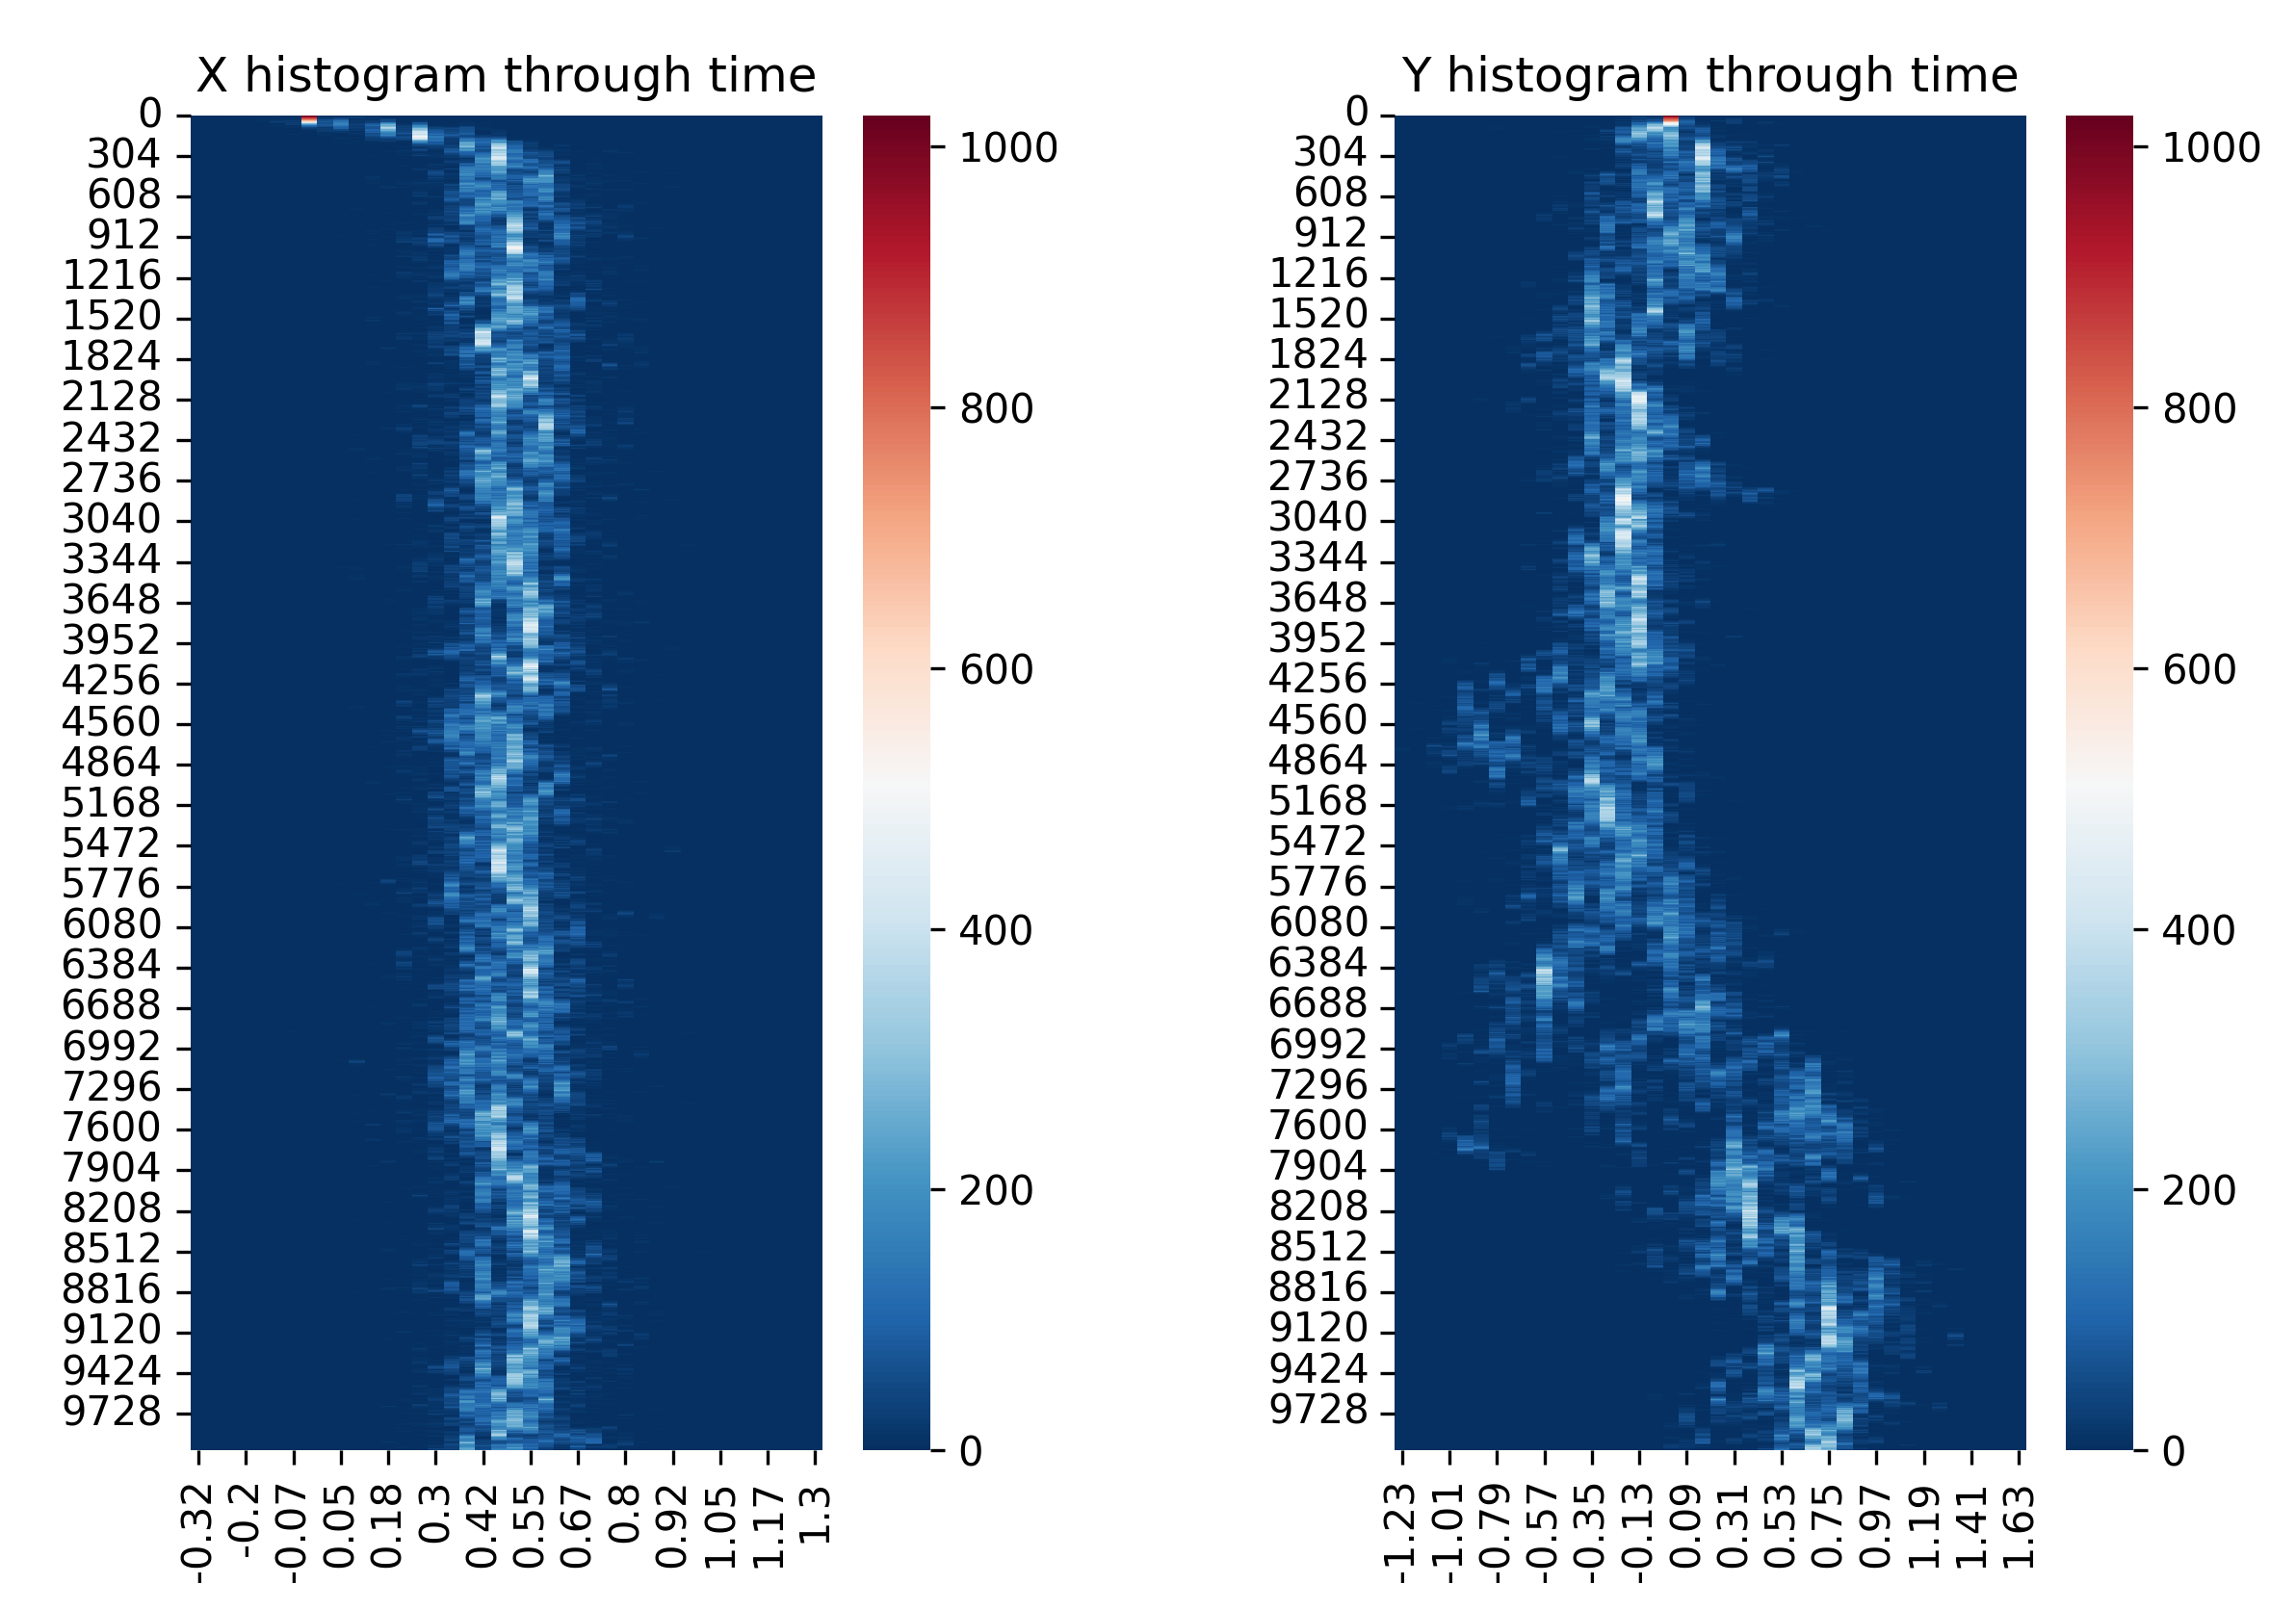
\includegraphics[scale=0.5]{10000} \\
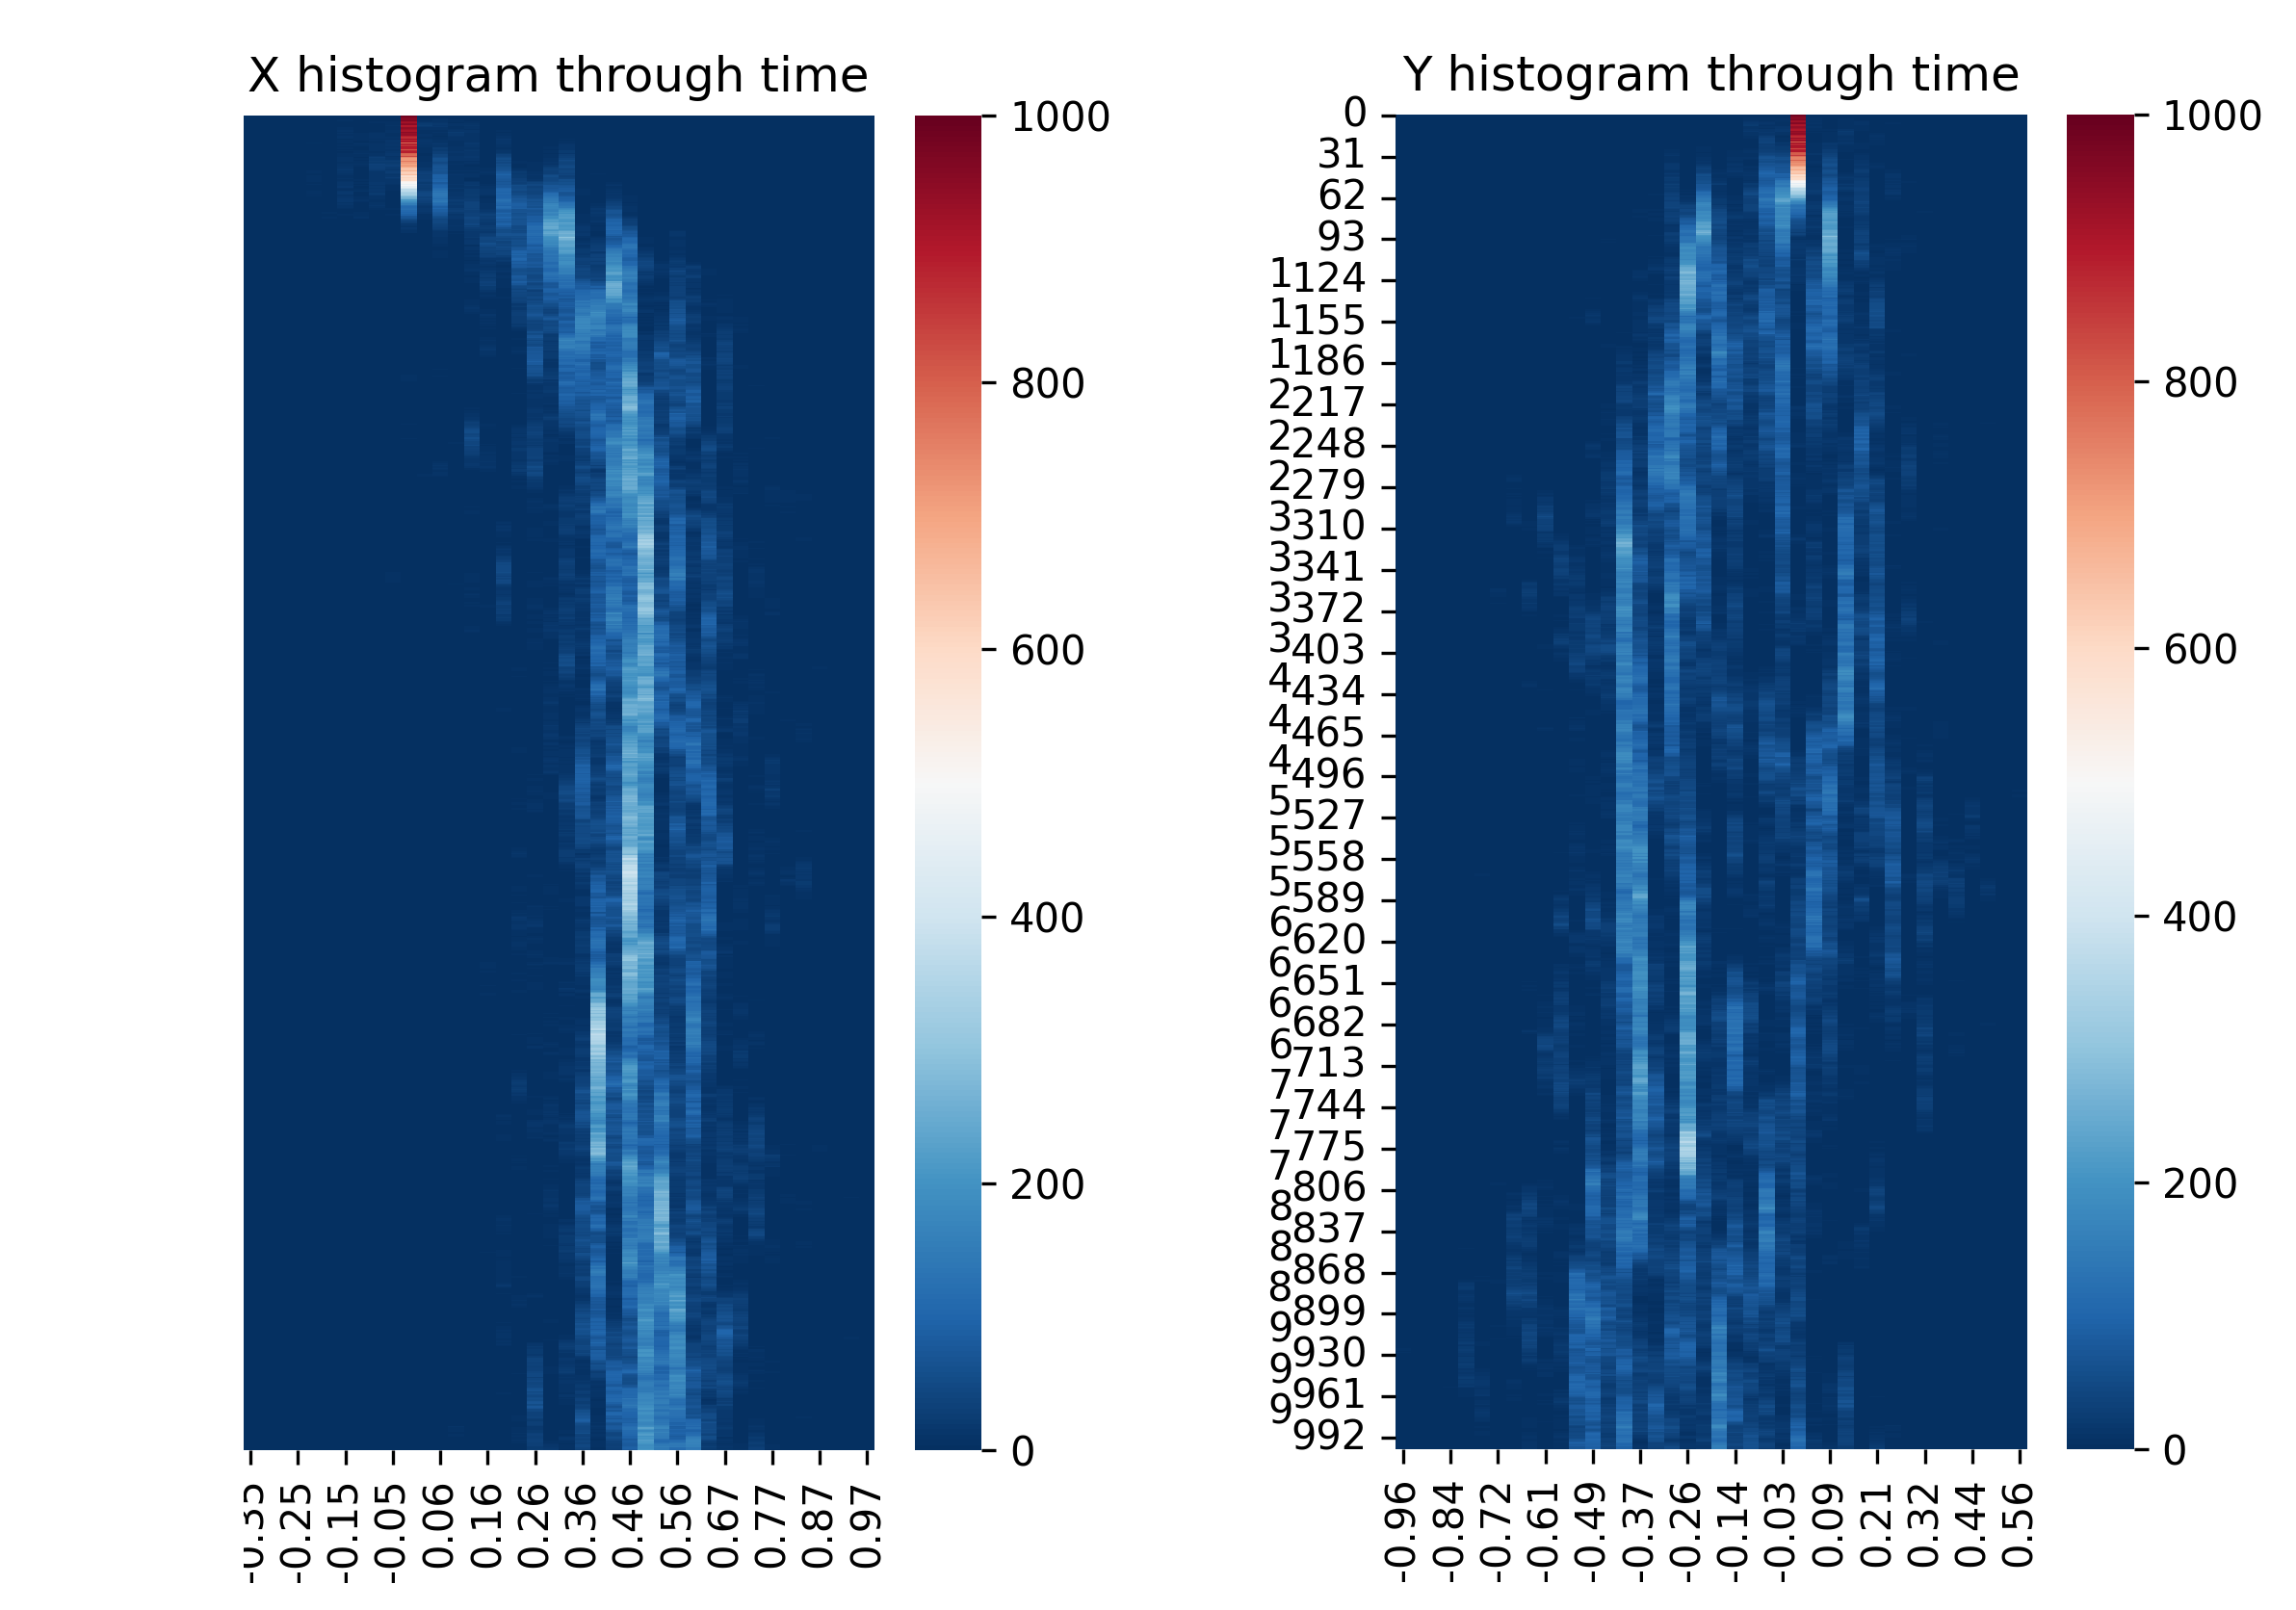
\includegraphics[scale=0.5]{1000} \\
\textit{Heatmaps of $X$ and $Y$ with recommended parameters for 1000 generations (top) and 10 000 generations (bottom)}
\end{center}

We can clearly see that $x$ stabilises around $0.5$ for these parameters.

\subsection{Checking $\beta$'s influence on $Y$}

From the formula defining death rate, the death rate of an individual is higher if $y$ is lower (resp. higher) than the mean value $\bar{Y}$ and lower when it's higher (resp. lower) than $\bar{Y}$, if $\beta$ is positive (resp. negative). \\
\vspace{5mm}

But as individuals with a low (resp. high) value of $y$ die out, the mean is pushed back to the right (resp. left), which happens in a continuous motion, until the influence of the directional selection term because negligeable when compared to the competition term. \\
\vspace{5mm}

\subsubsection{Positive versus negative value of $\beta$}

To start, we checked that positive values of $\beta$ pushed $y$ values towards more positive values and that negative values of $\beta$ pushed $y$ values towards more negative values : \\

\begin{center}
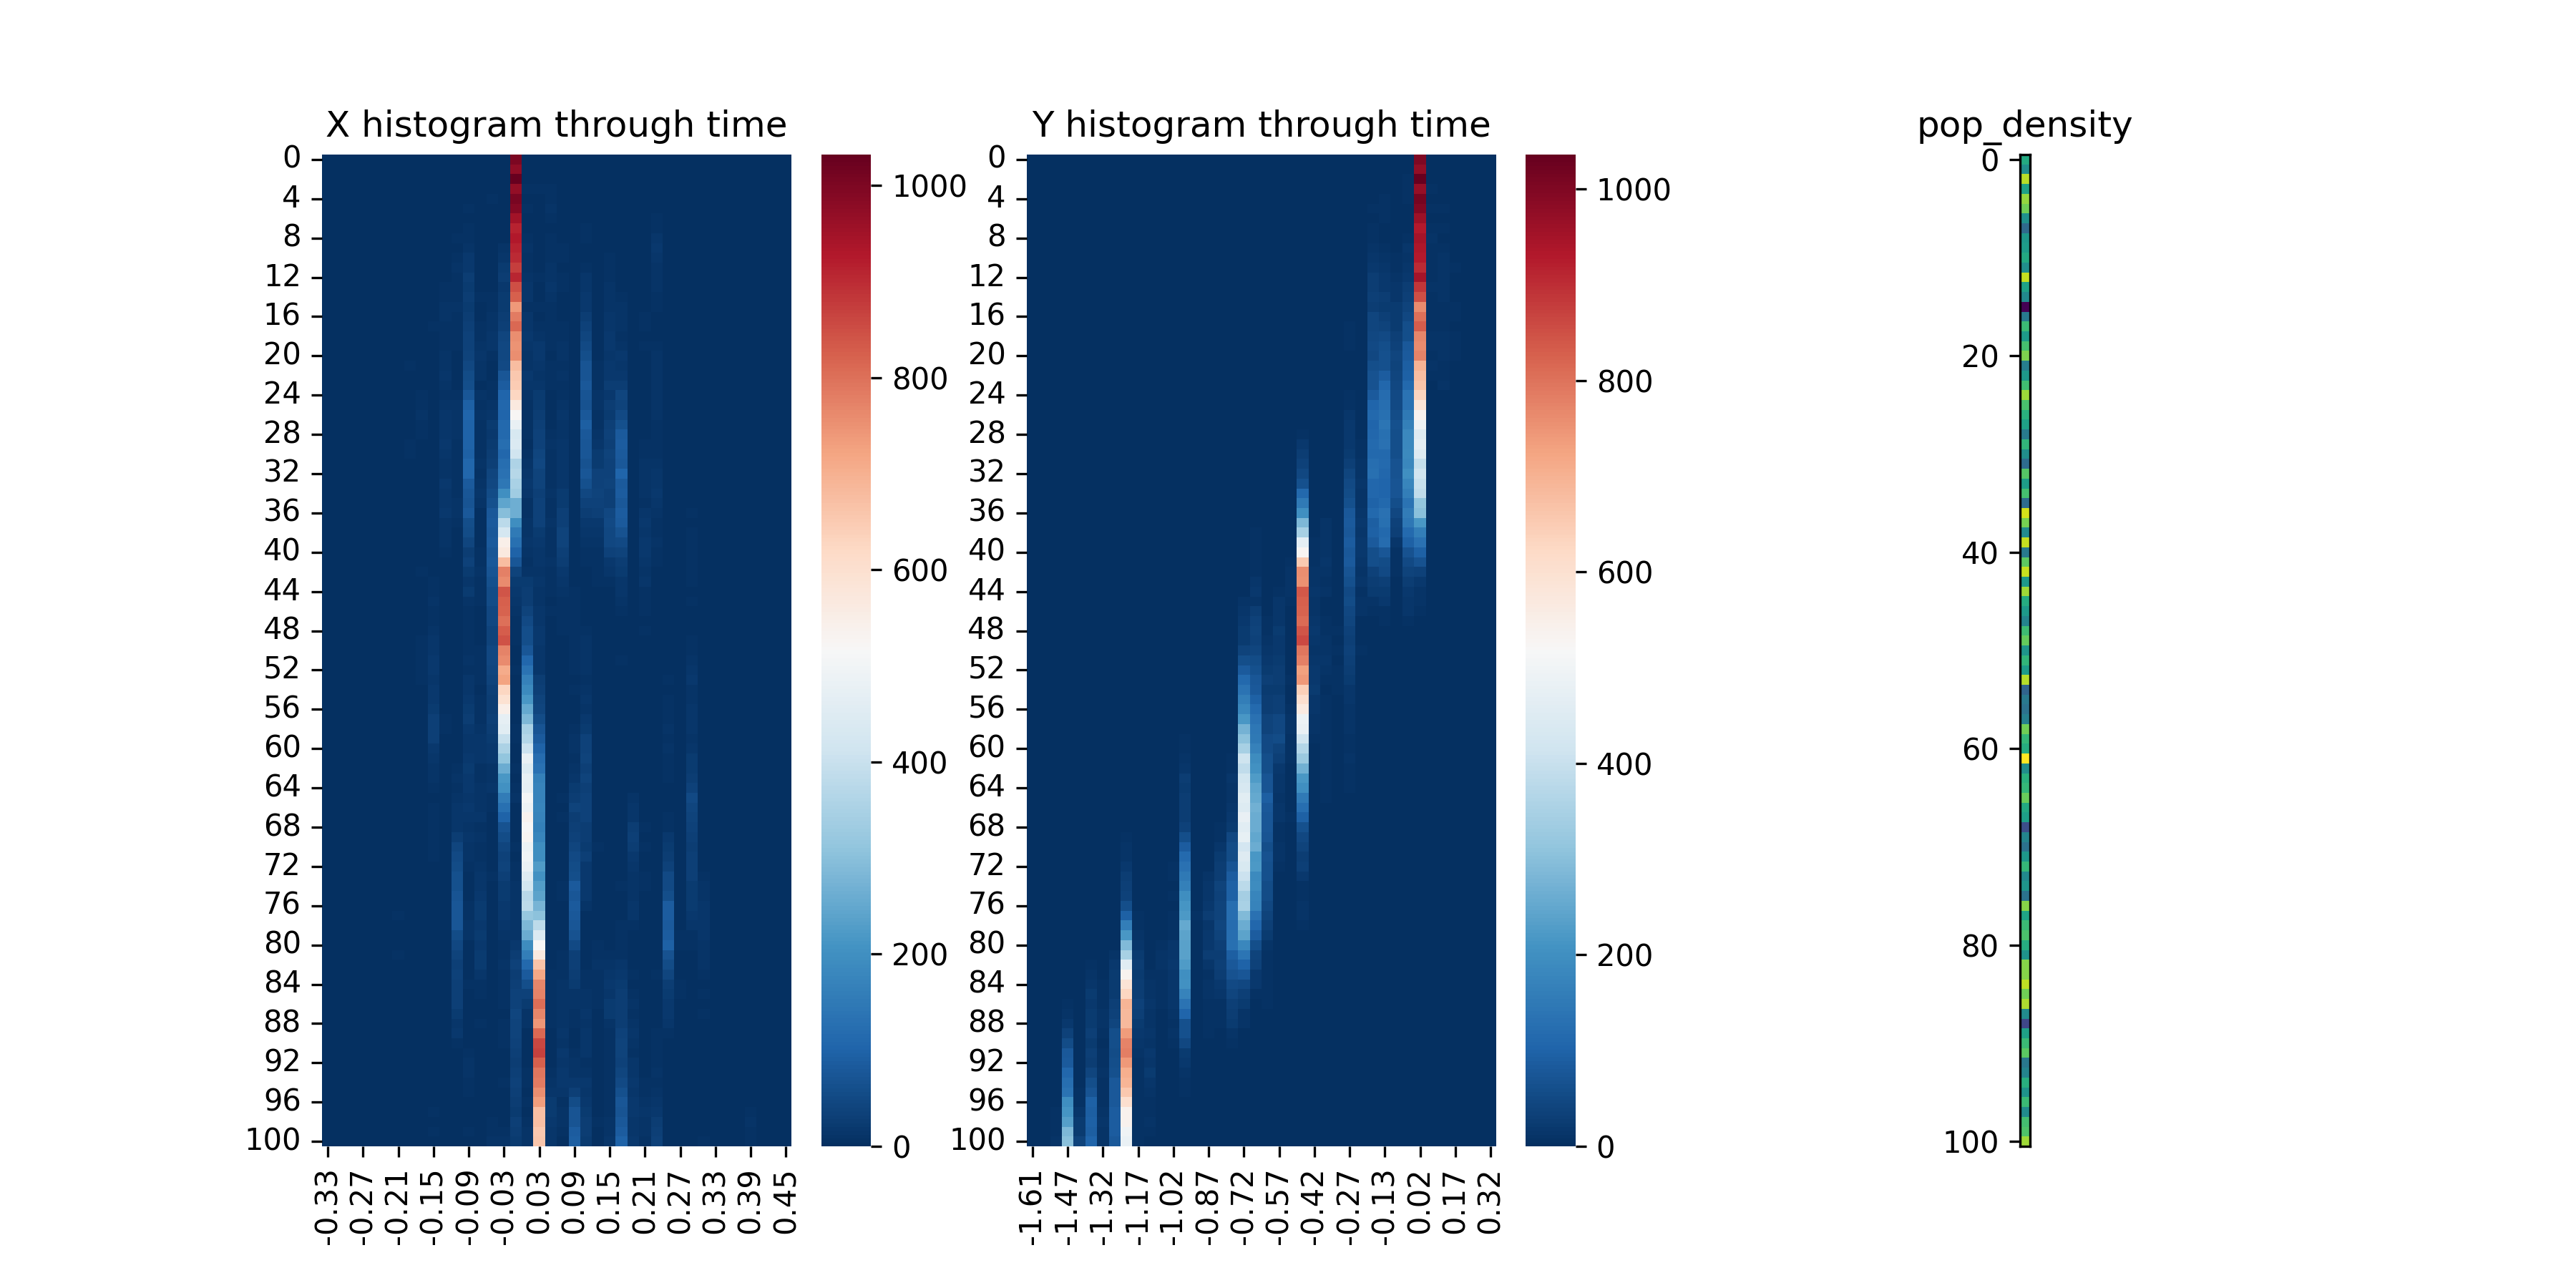
\includegraphics[scale=0.37]{beta=-1} 
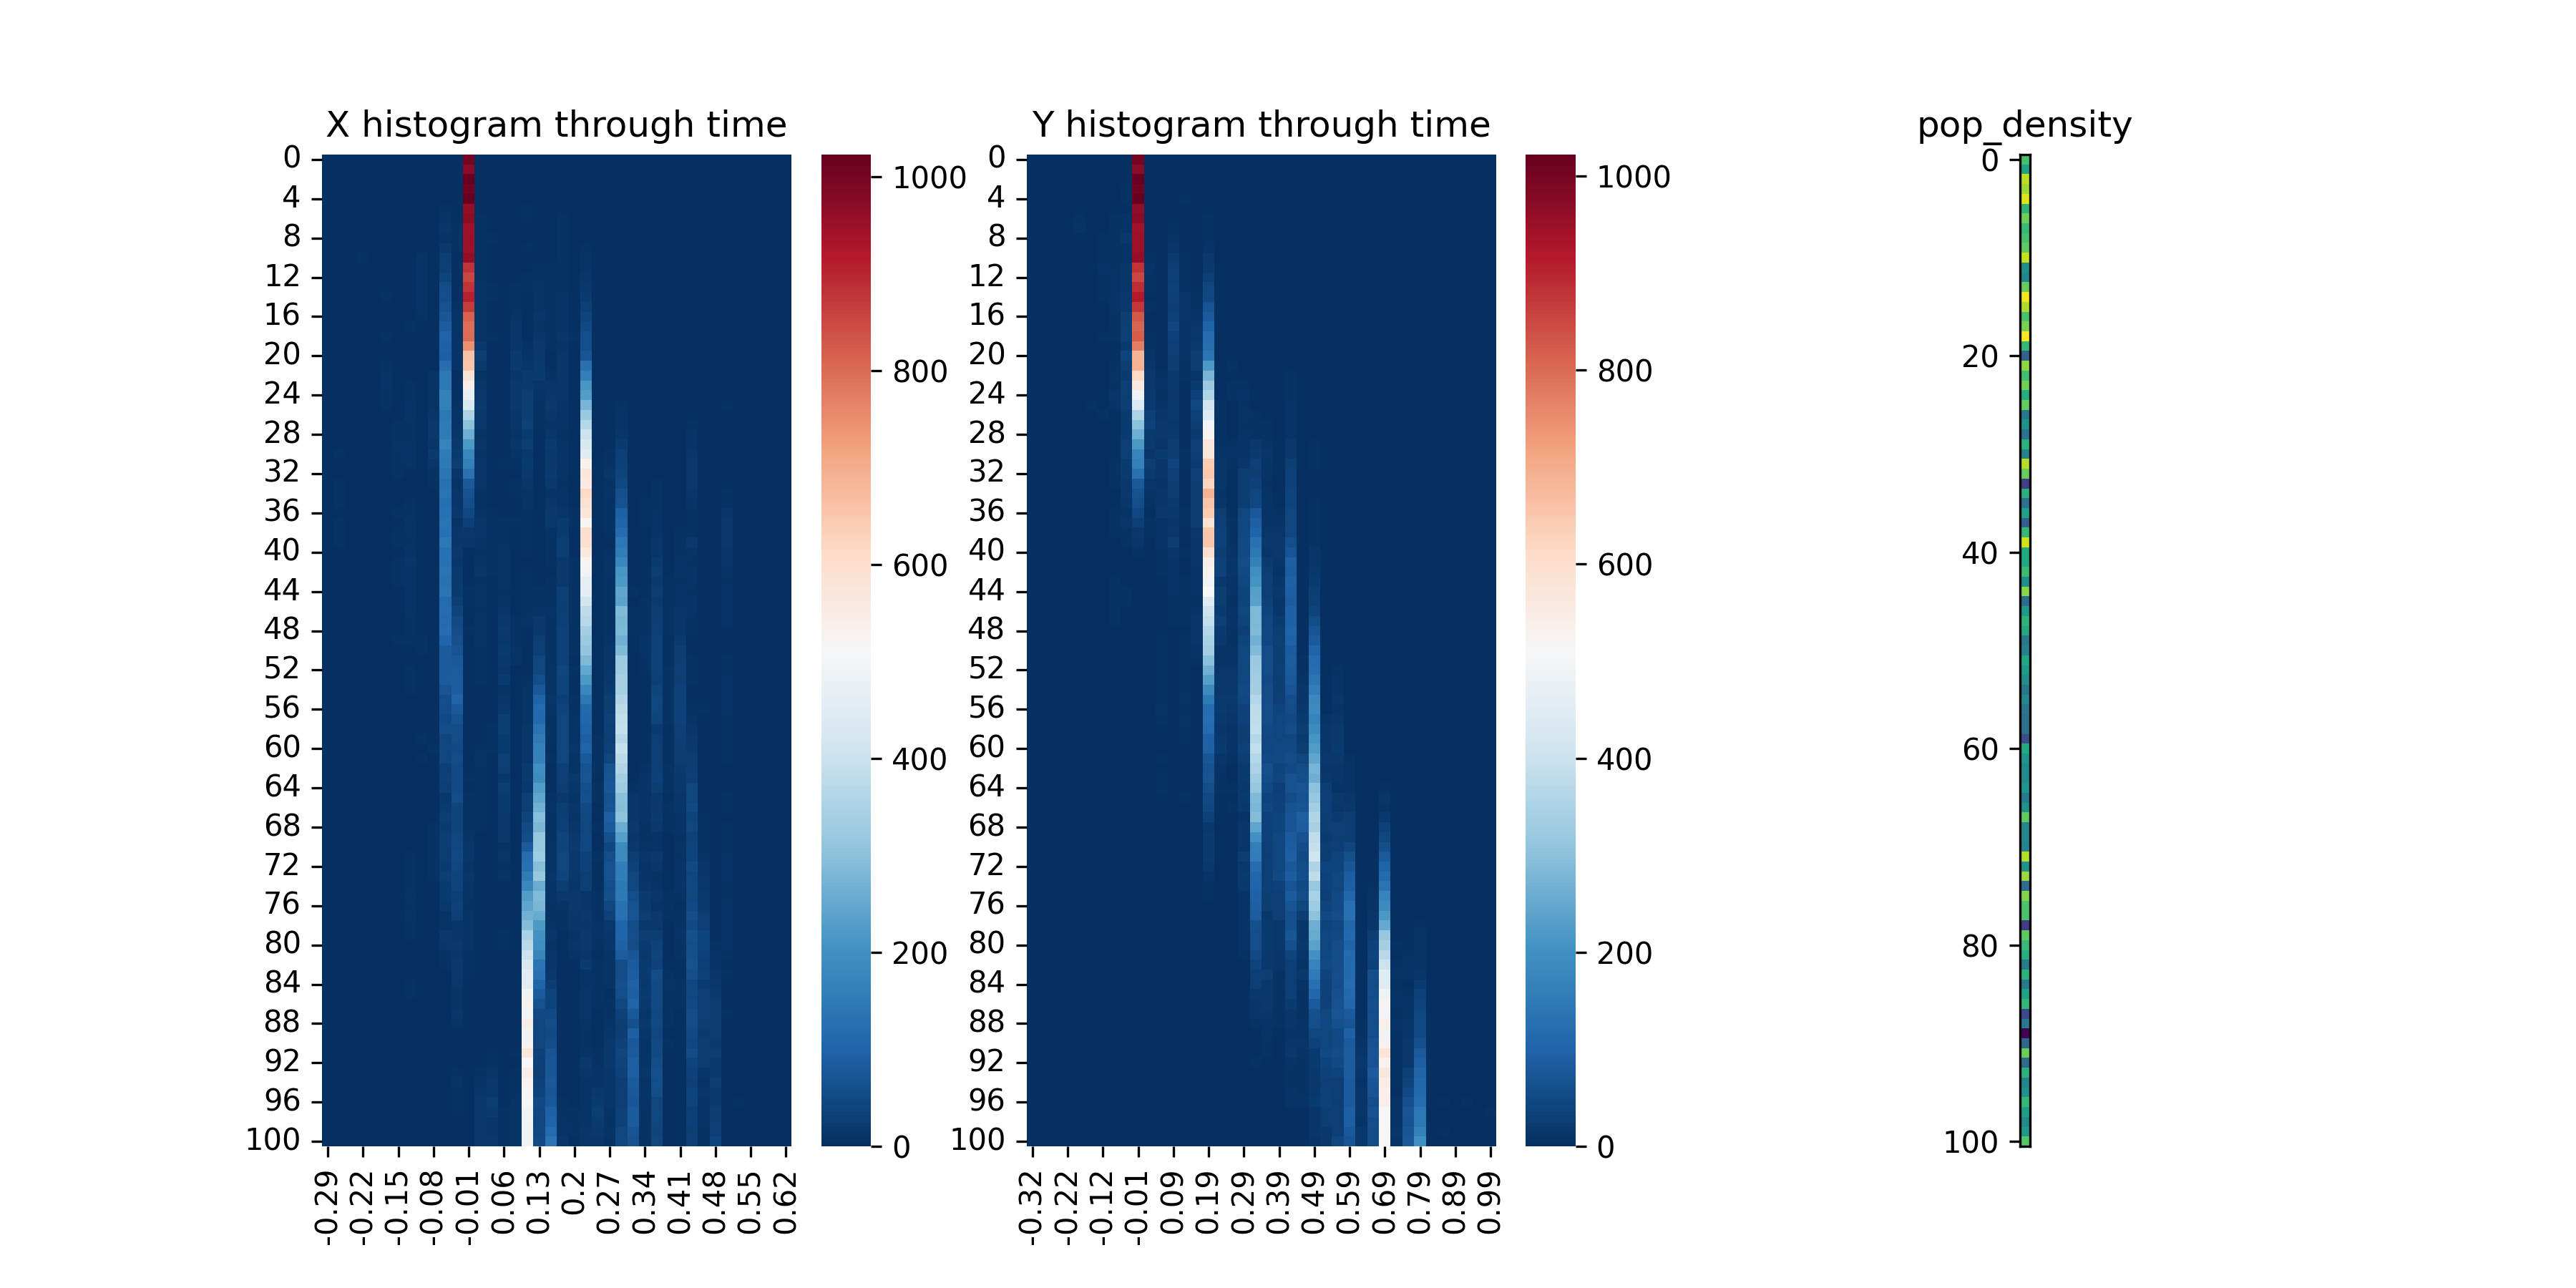
\includegraphics[scale=0.37]{beta=1} \\
\textit{Heatmaps of $X$ and $Y$ for $\beta = -1$ (top) and $\beta = 1$ (bottom)}
\end{center}
\vspace{5mm}

Indeed, we see it's pushed to the left / right according to the value of $\beta$. \\

\subsubsection{Comparing $\beta = 1$ with $\beta = 2$}

We expect to see $Y$ reach further to the right for $\beta = 2$ than for $\beta = 1$. \\
\begin{center}
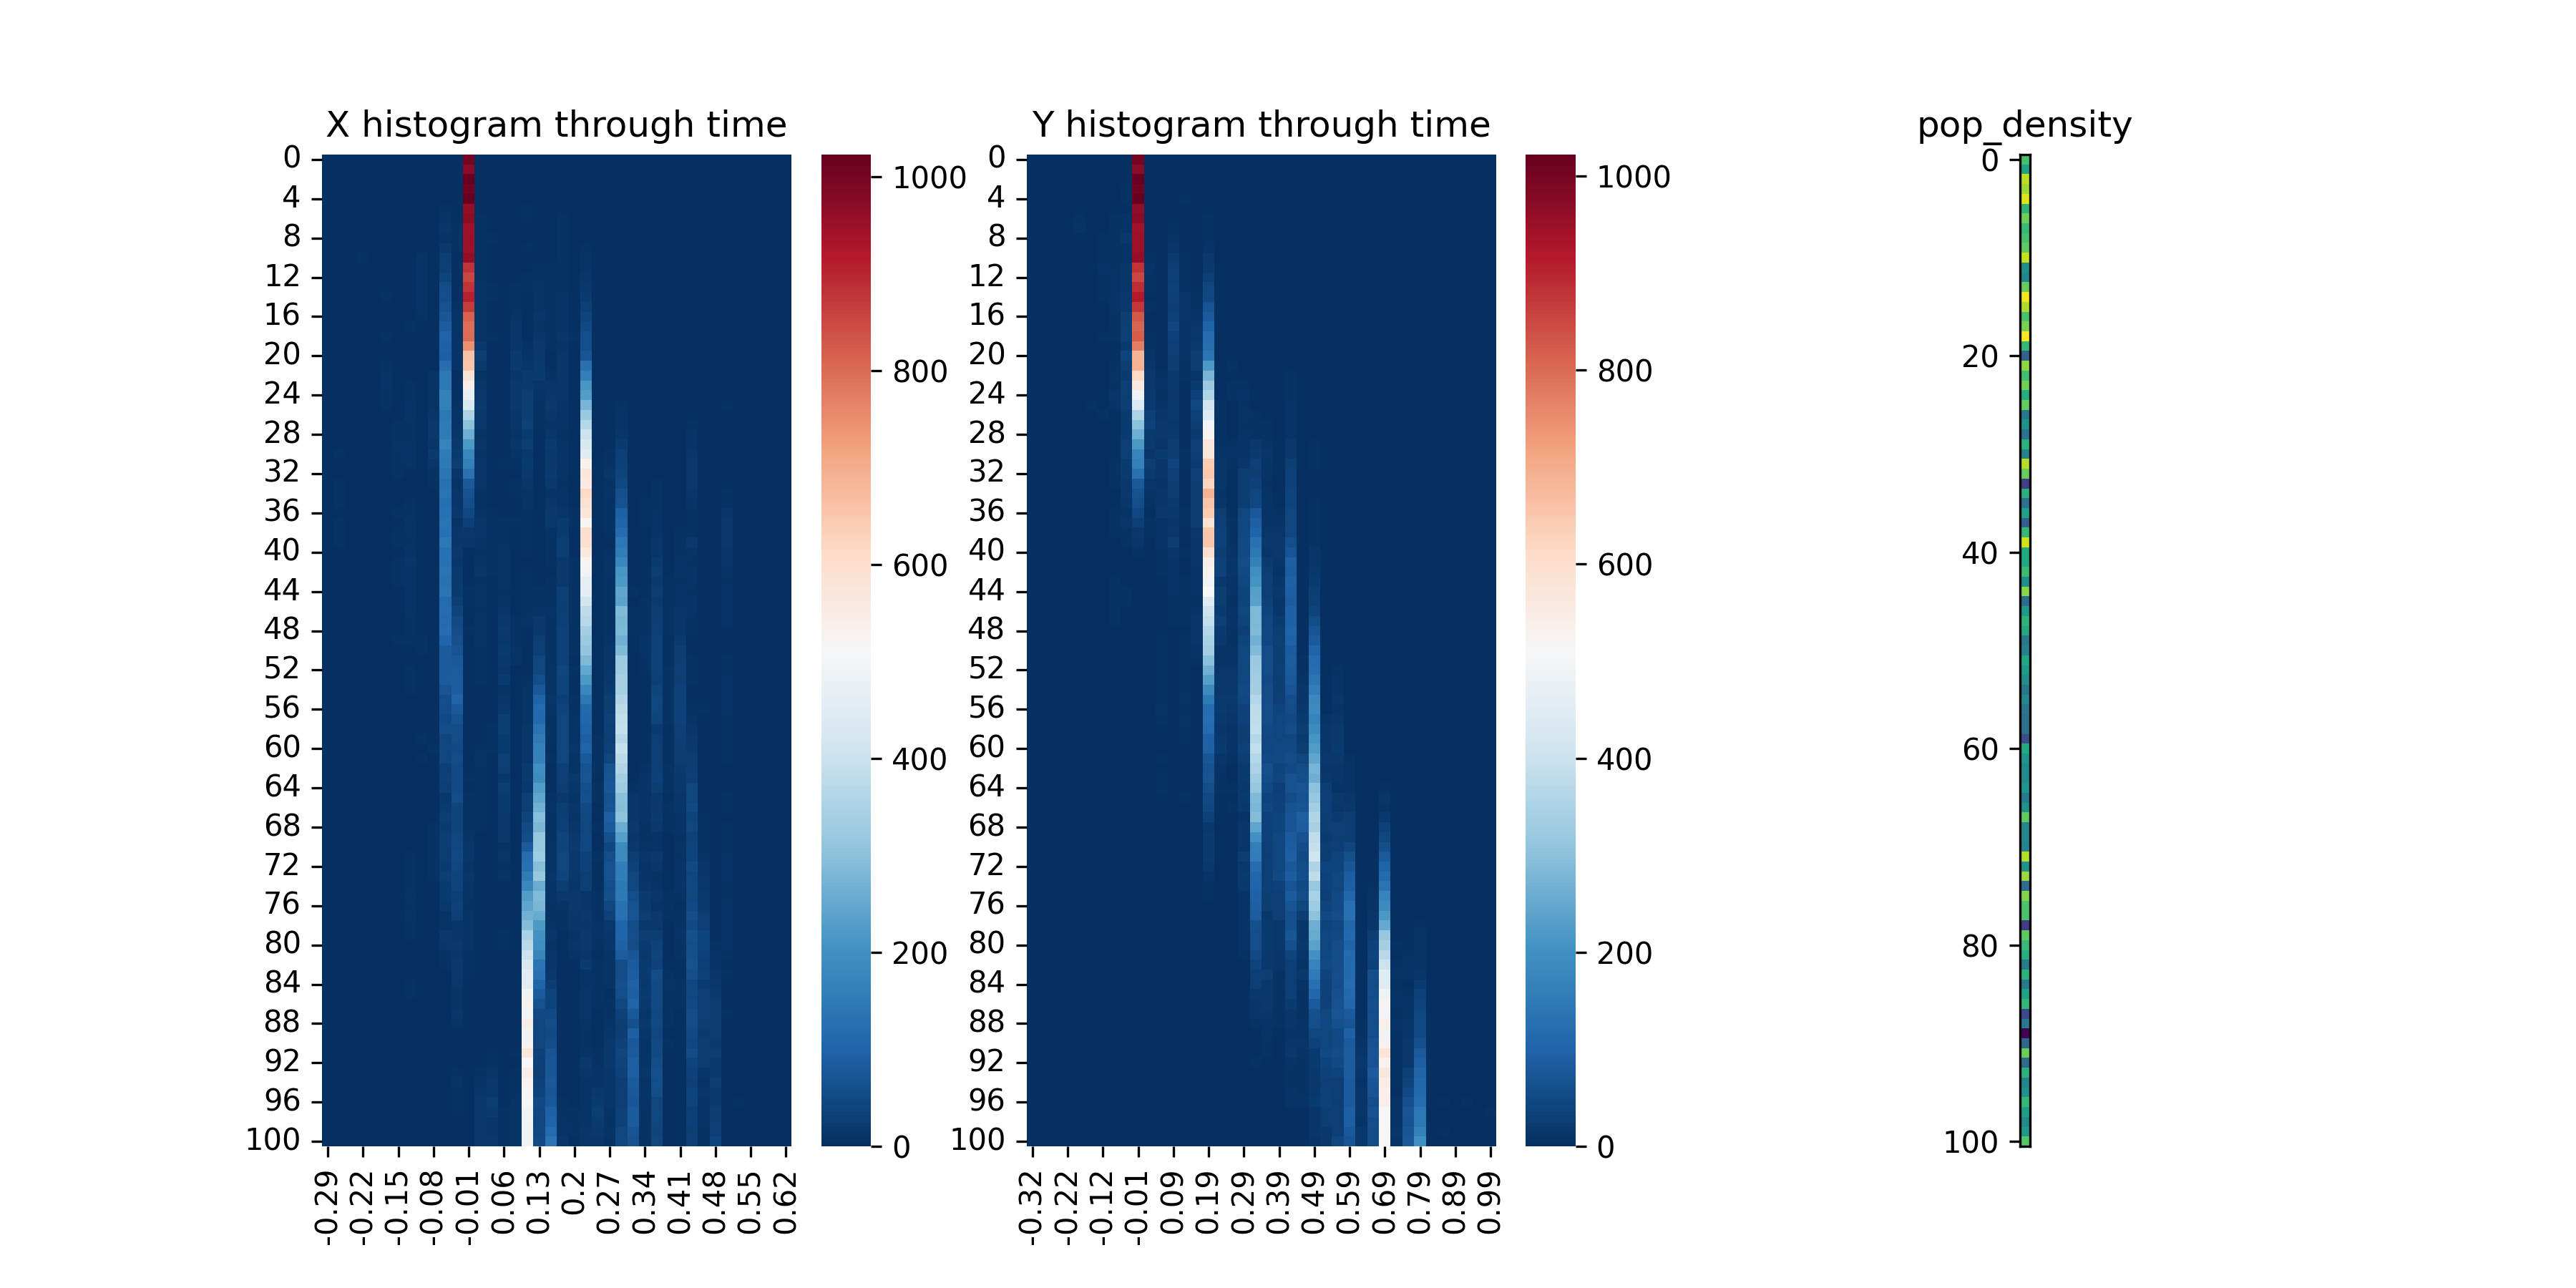
\includegraphics[scale=0.37]{beta=1}
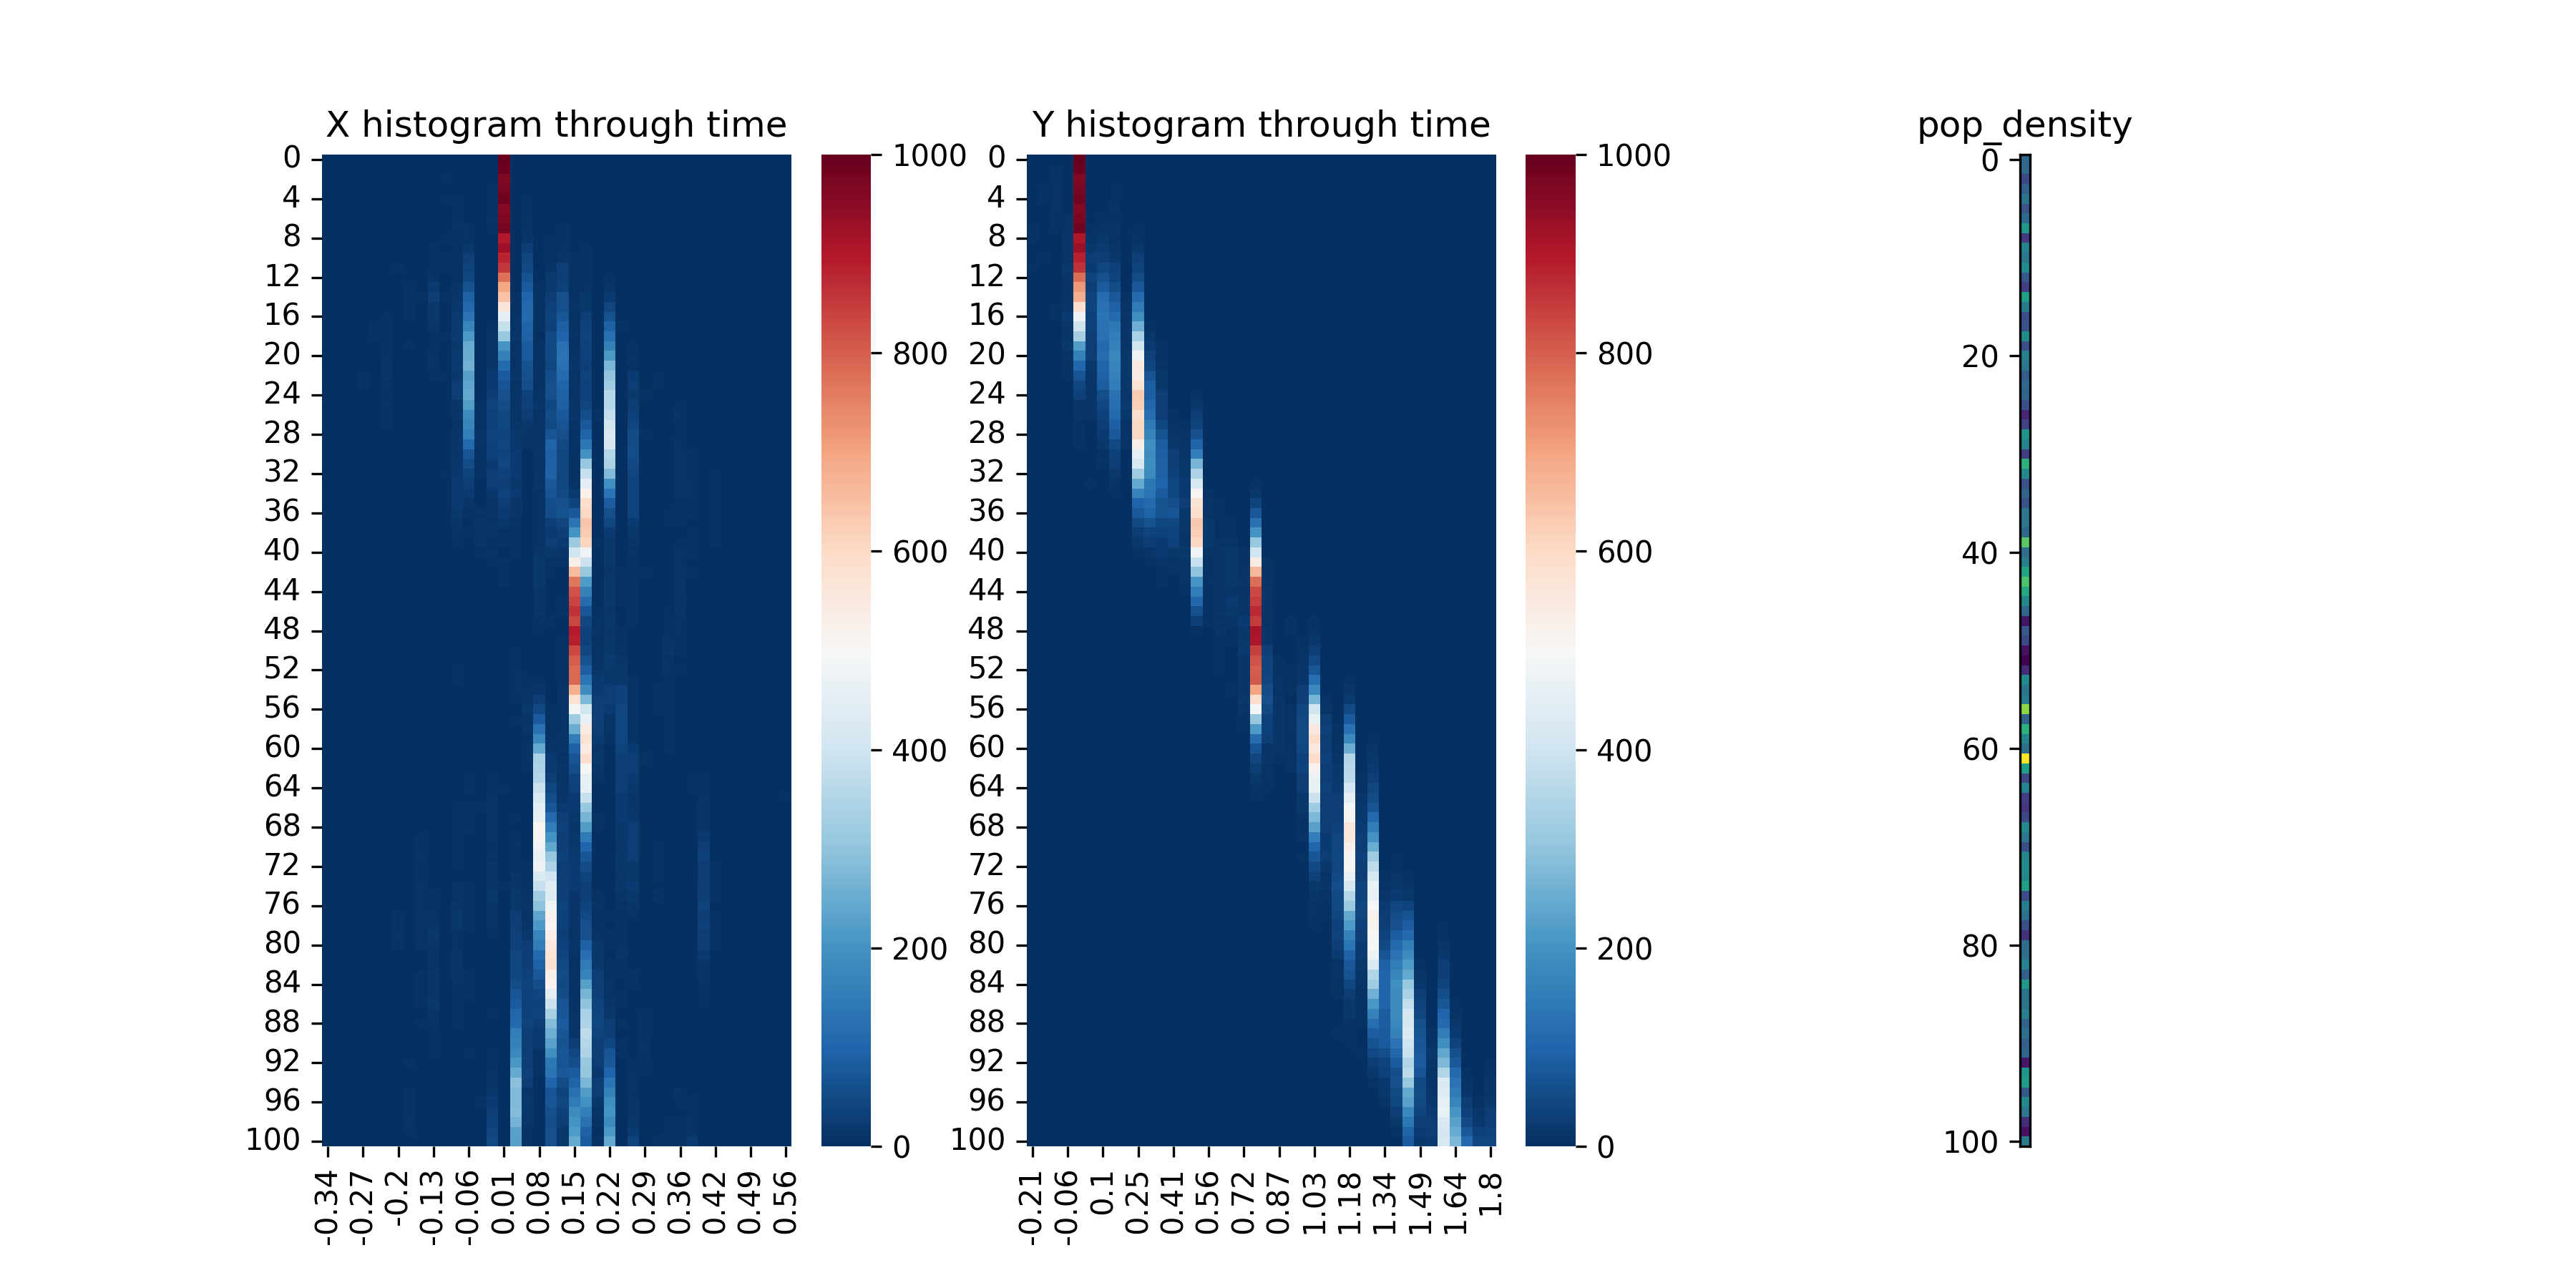
\includegraphics[scale=0.37]{beta=2} \\
\textit{Heatmaps of $X$ and $Y$ for $\beta = 1$ (top) and $\beta = 2$ (bottom)}
\end{center}
\vspace{5mm}

Of course, we do see $Y$ values reach about twice as far, as expected. \\
\vspace{5mm}

\subsubsection{Letting the simulation run for longer with $\beta = 100$}

\begin{center}
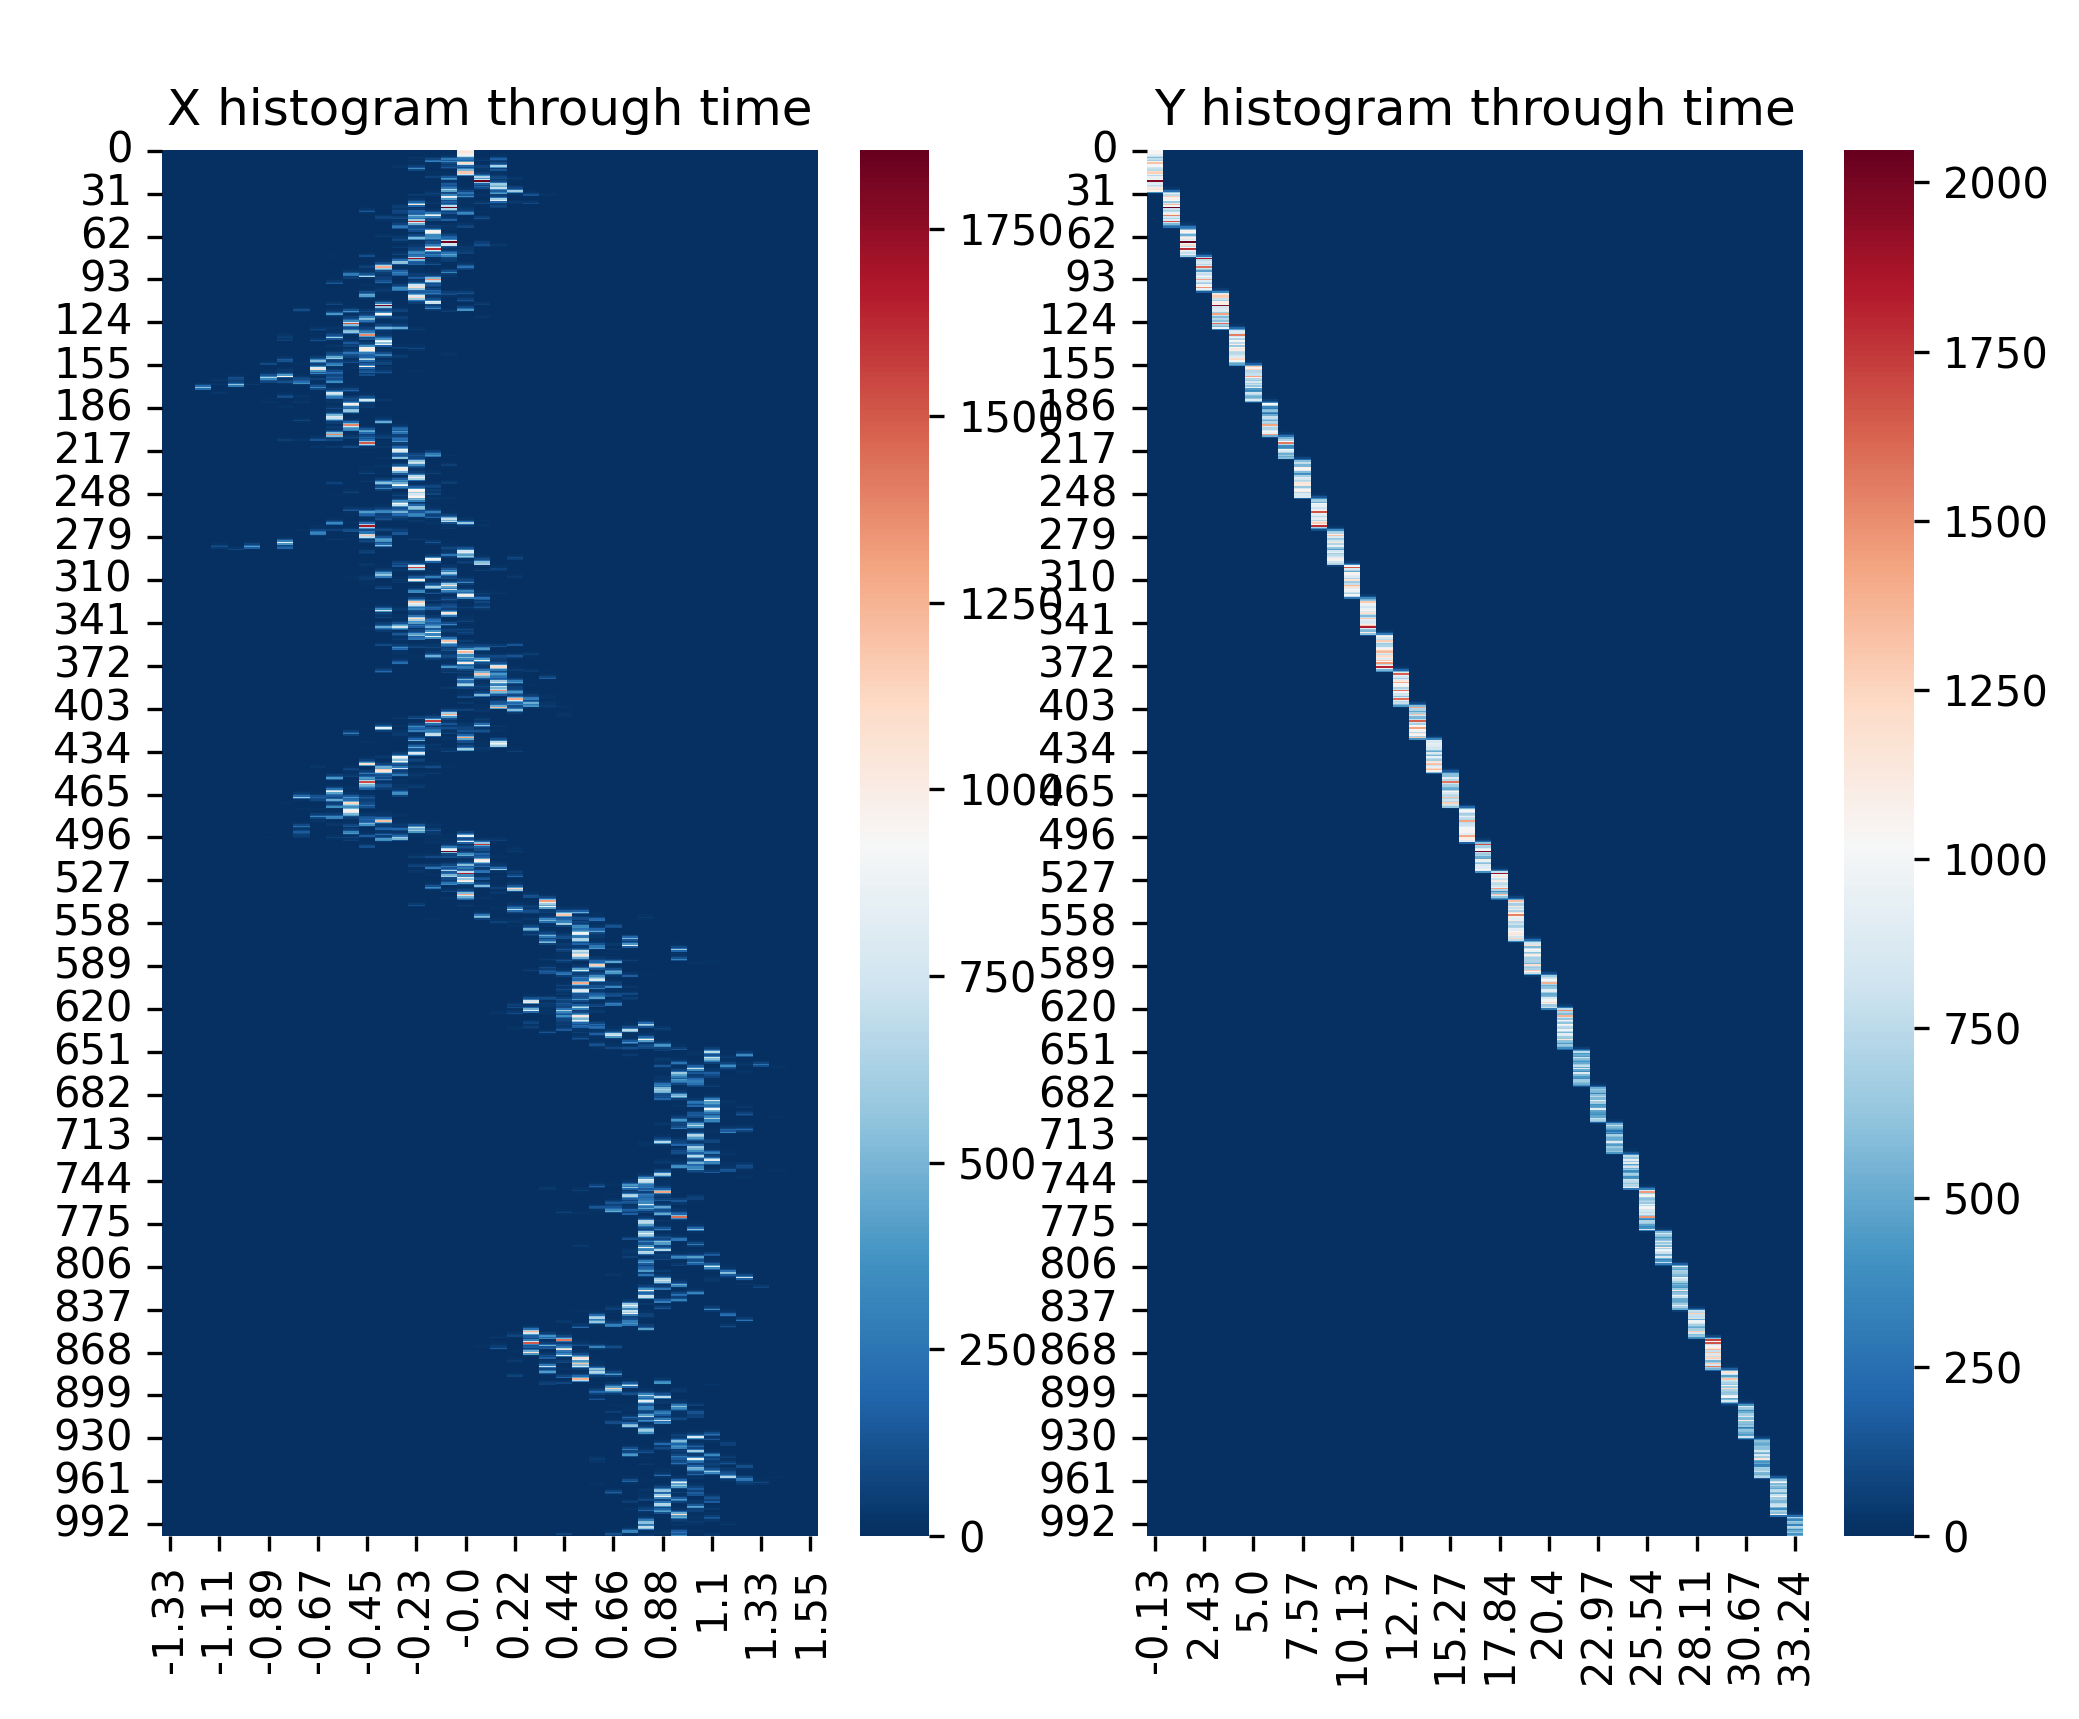
\includegraphics[scale=0.5]{beta=100}
\textit{Heatmaps of $X$ and $Y$ for $\beta = 100$ over $1000$ generations}
\end{center}

In this extreme case, we can actually see more variation in $X$ because of the longer simulation time, and $Y$'s behaviour remains completely predictable, making it as far as about $33$au.

\subsection{Showing how $\mu$ and $K_0$ affects simulation evolution}

\subsubsection{$\mu$ increase leads to accelerated effects}
We increased mutation rate $\mu$ to increase how much change can be perceived in each generation, and, in turn, effectively how fast the transitions occur. \\
\vspace{5mm}

\begin{center}
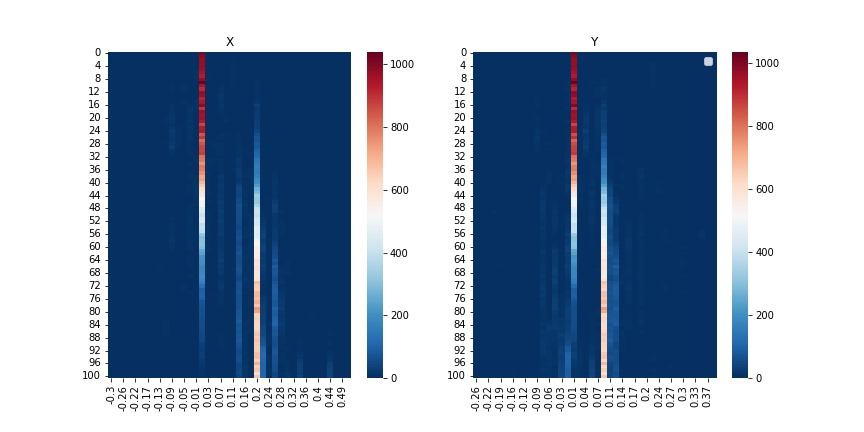
\includegraphics[scale=0.37]{heatmap_mu_0.005}
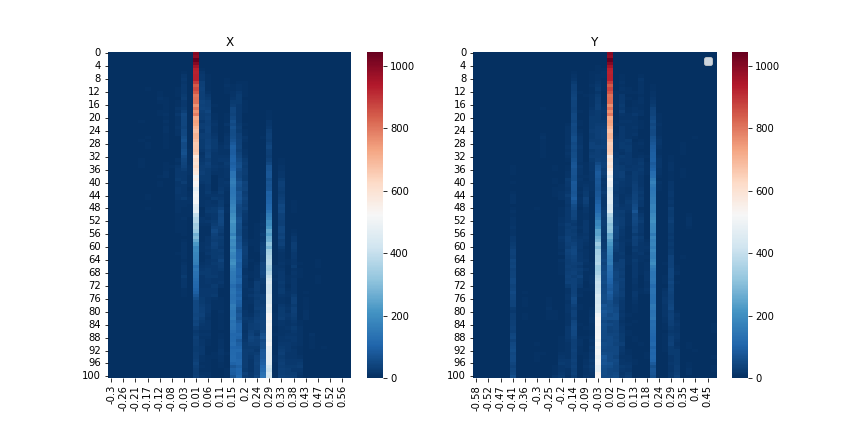
\includegraphics[scale=0.37]{heatmap_mu_0.01}
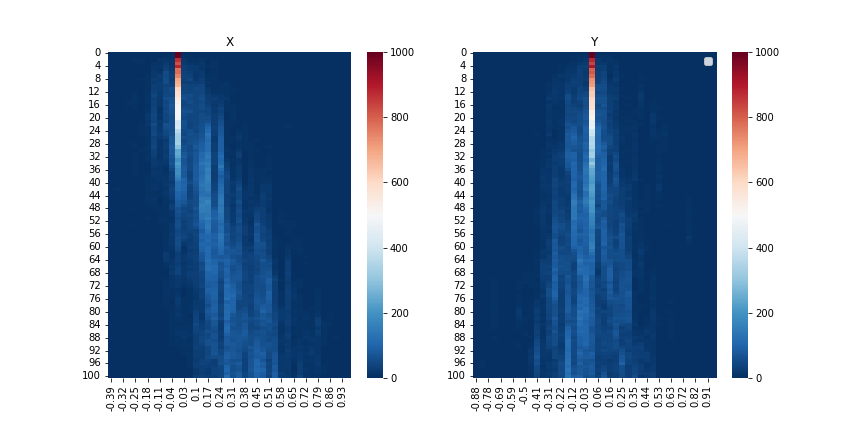
\includegraphics[scale=0.37]{heatmap_mu_0.05}
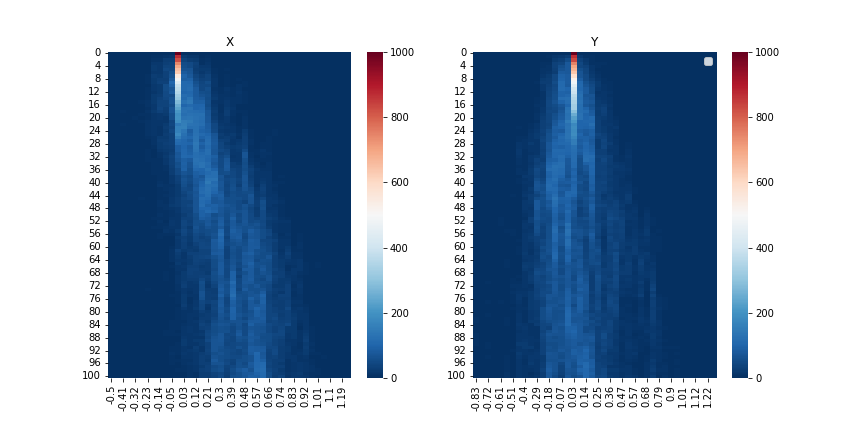
\includegraphics[scale=0.37]{heatmap_mu_0.1}
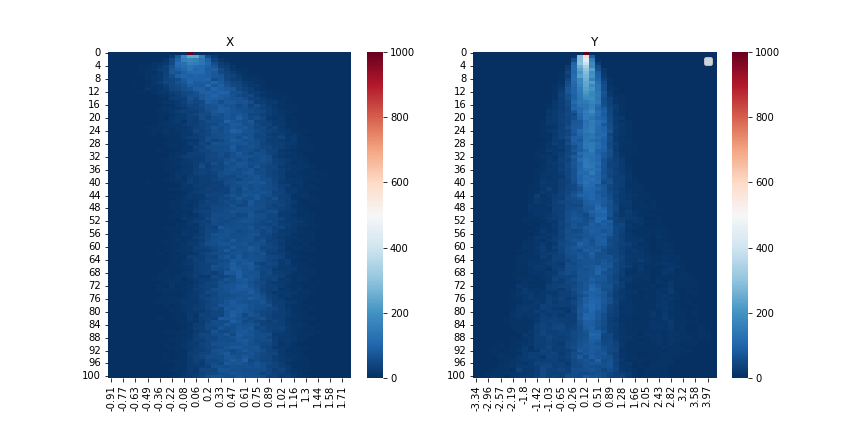
\includegraphics[scale=0.37]{heatmap_mu_1.0} \\
\textit{Heatmaps of $X$ and $Y$ for $\mu \in \lbrace 0.005,0.01,0.05,0.1,1 \rbrace$ (top to bottom)}
\end{center}

We can clearly see that the increasing values of mutation rates are causing more and more variation to occur each generation, causing this sort of blur effect over time when $\mu$ is large. This naturally speeds up most effects that arise from mutation, as we can see when we set $\beta$ to 1 and $\mu$ to $0.2$ : \\

\begin{center}
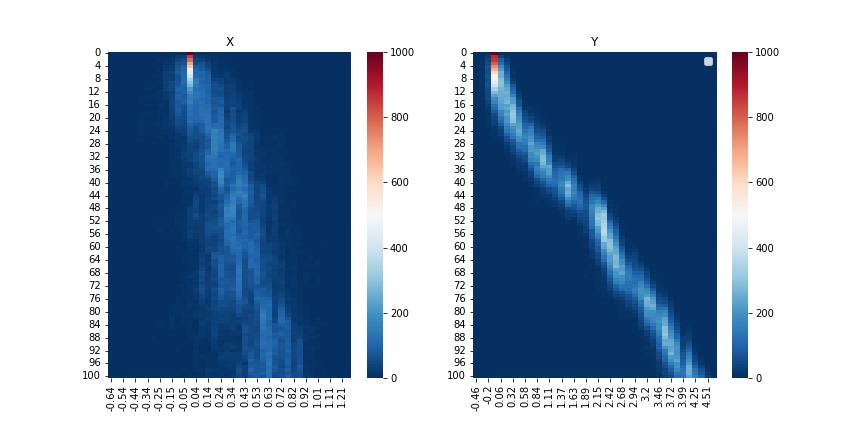
\includegraphics[scale=0.37]{beta=1mu=0.15}
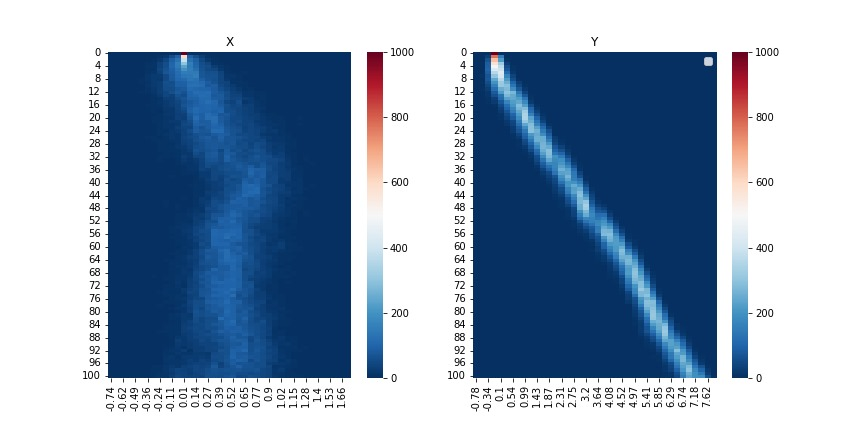
\includegraphics[scale=0.37]{beta=1mu=0.5} \\
\textit{Heatmaps of $X$ and $Y$ for $\beta = 1$ and $\mu = 0.15$ (top) and $\mu = 0.5$ (bottom)}
\end{center}

We can clearly see how $Y$'s linear movement is "blurred" by the higher mutation rate and increase faster as $\mu$ increase. \\
\vspace{5mm}

\subsubsection{$K_0$ increase leads to decelerated effects}

Similarly, an increase population size $K_0$ will cause the effects to happen slower, as we can see in the following graph : \\
\vspace{5mm}

\begin{center}
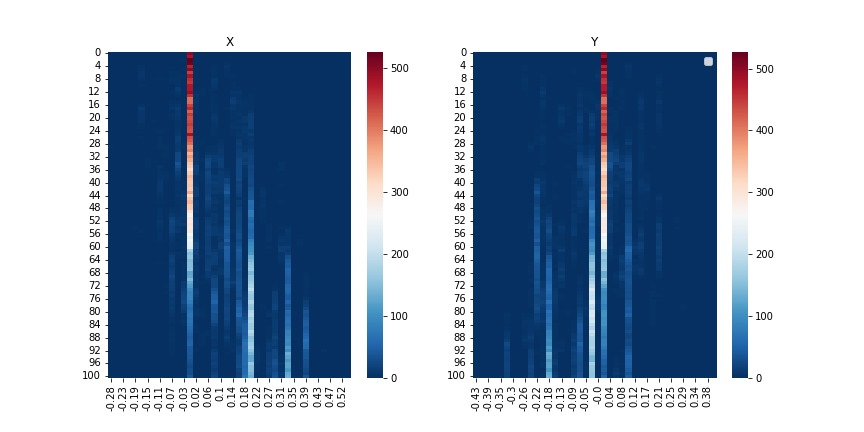
\includegraphics[scale=0.37]{500k0}
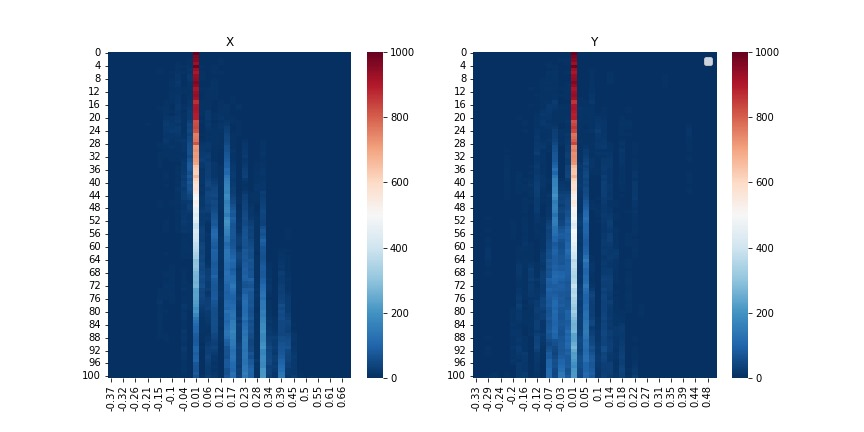
\includegraphics[scale=0.37]{1000k0}
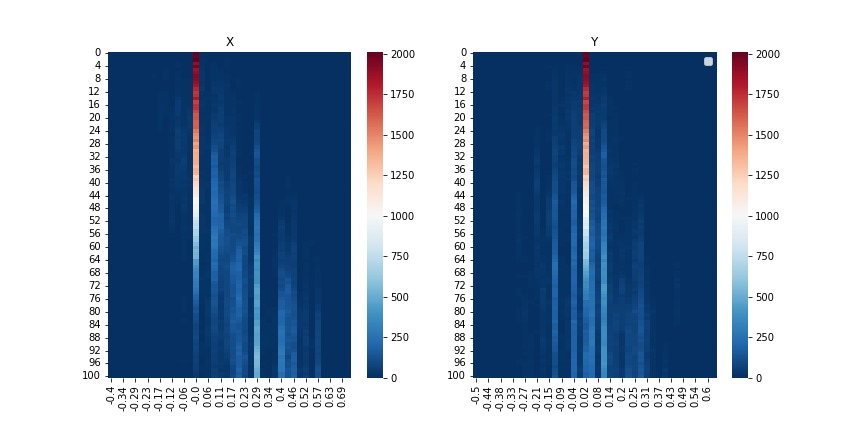
\includegraphics[scale=0.37]{2000k0} \\
\textit{Heatmaps of $X$ and $Y$ for $K_0 \in \lbrace 500, 1000, 2000 \rbrace$ (top to bottom)}
\end{center}

Checking what effect this has for $\beta = 1$ : \\

\begin{center}
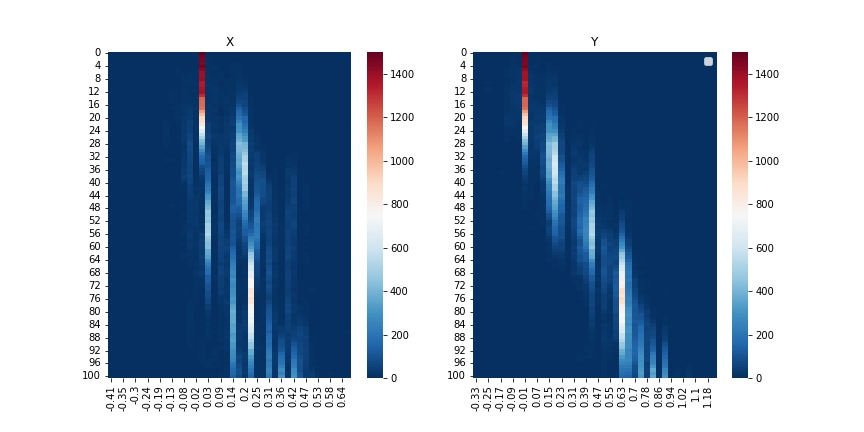
\includegraphics[scale=0.37]{beta=1k0=1500} 
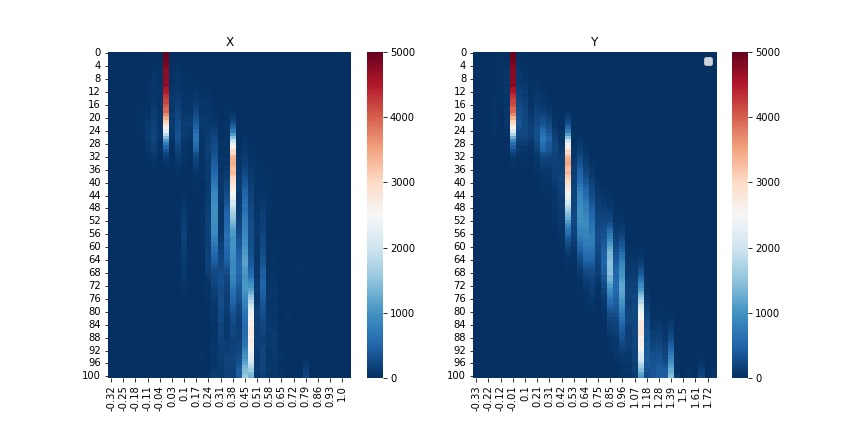
\includegraphics[scale=0.37]{beta=1k0=5000} \\
\textit{Heatmaps of $X$ and $Y$ for $\beta = 1$ and $K_0 = 1500$ (top) and $K_0 = 2000$ (bottom)}
\end{center}


\subsection{Showing $\sigma$ and $x_0$ sweeps}

We didn't really touch on initial conditions that much yet. We'll only sweep over $x_0$, but we'll combine it with the competition Gaussian's variance $\sigma_c^2$, and then resource exploitation variance $\sigma_k^2$. \\
\vspace{5mm}

\subsubsection{$\sigma_c$ sweeps}

\begin{center}
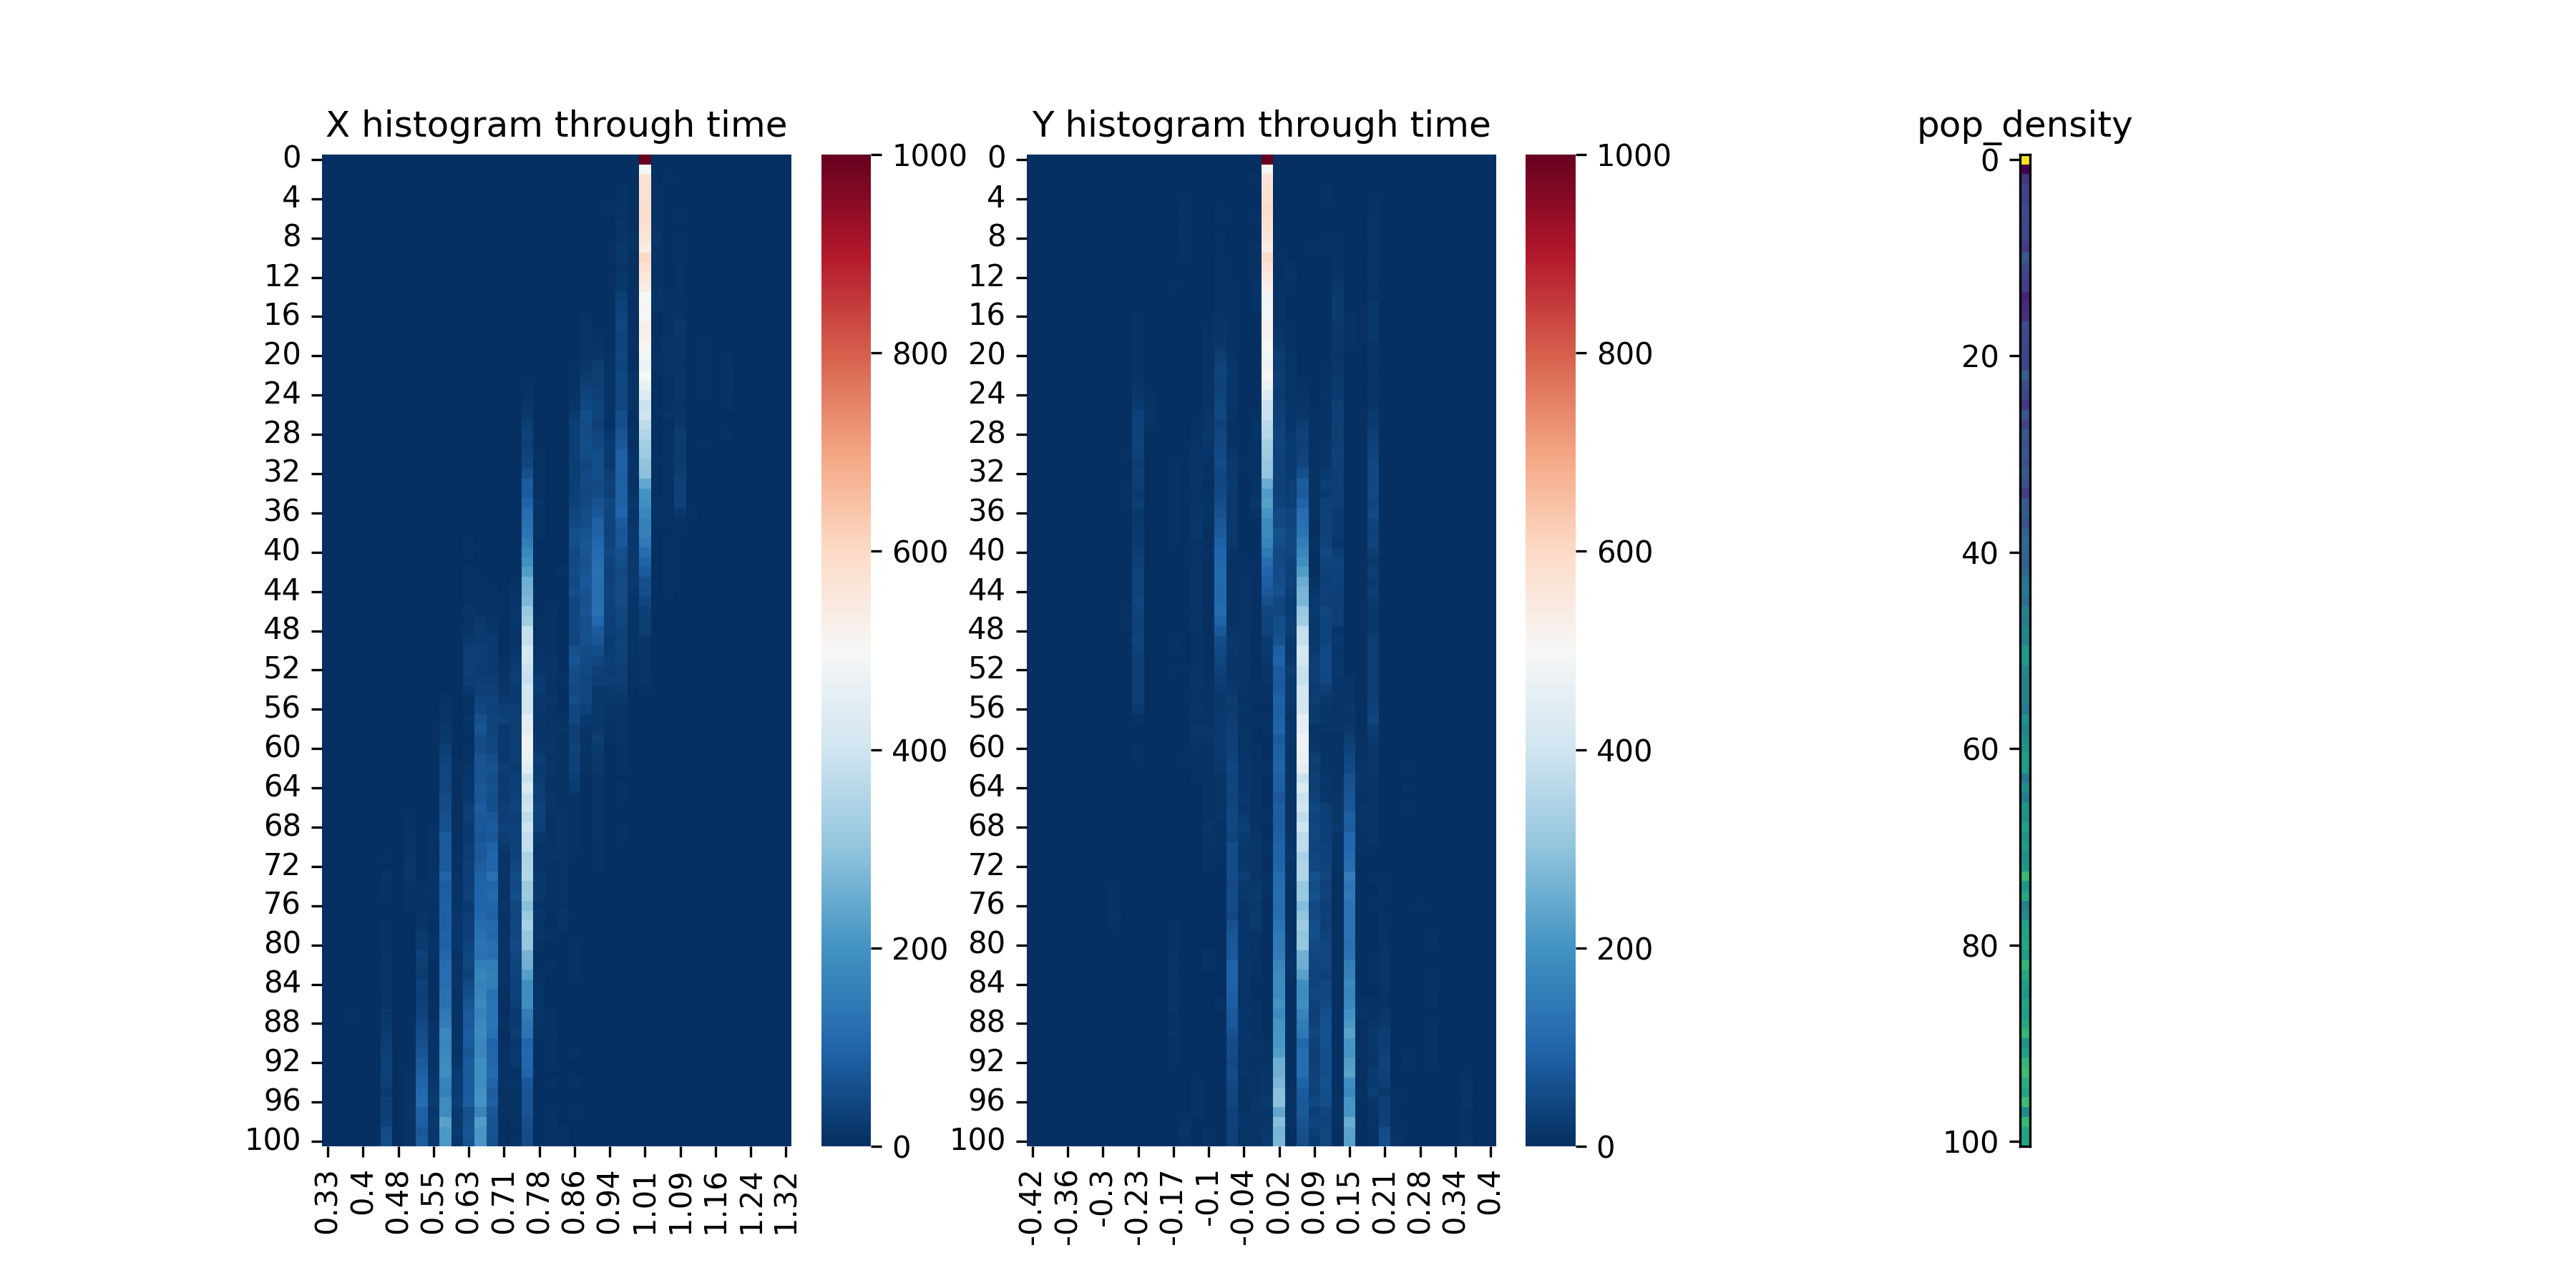
\includegraphics[scale=0.37]{x0_sc_sweep_(1.0)_(1)}
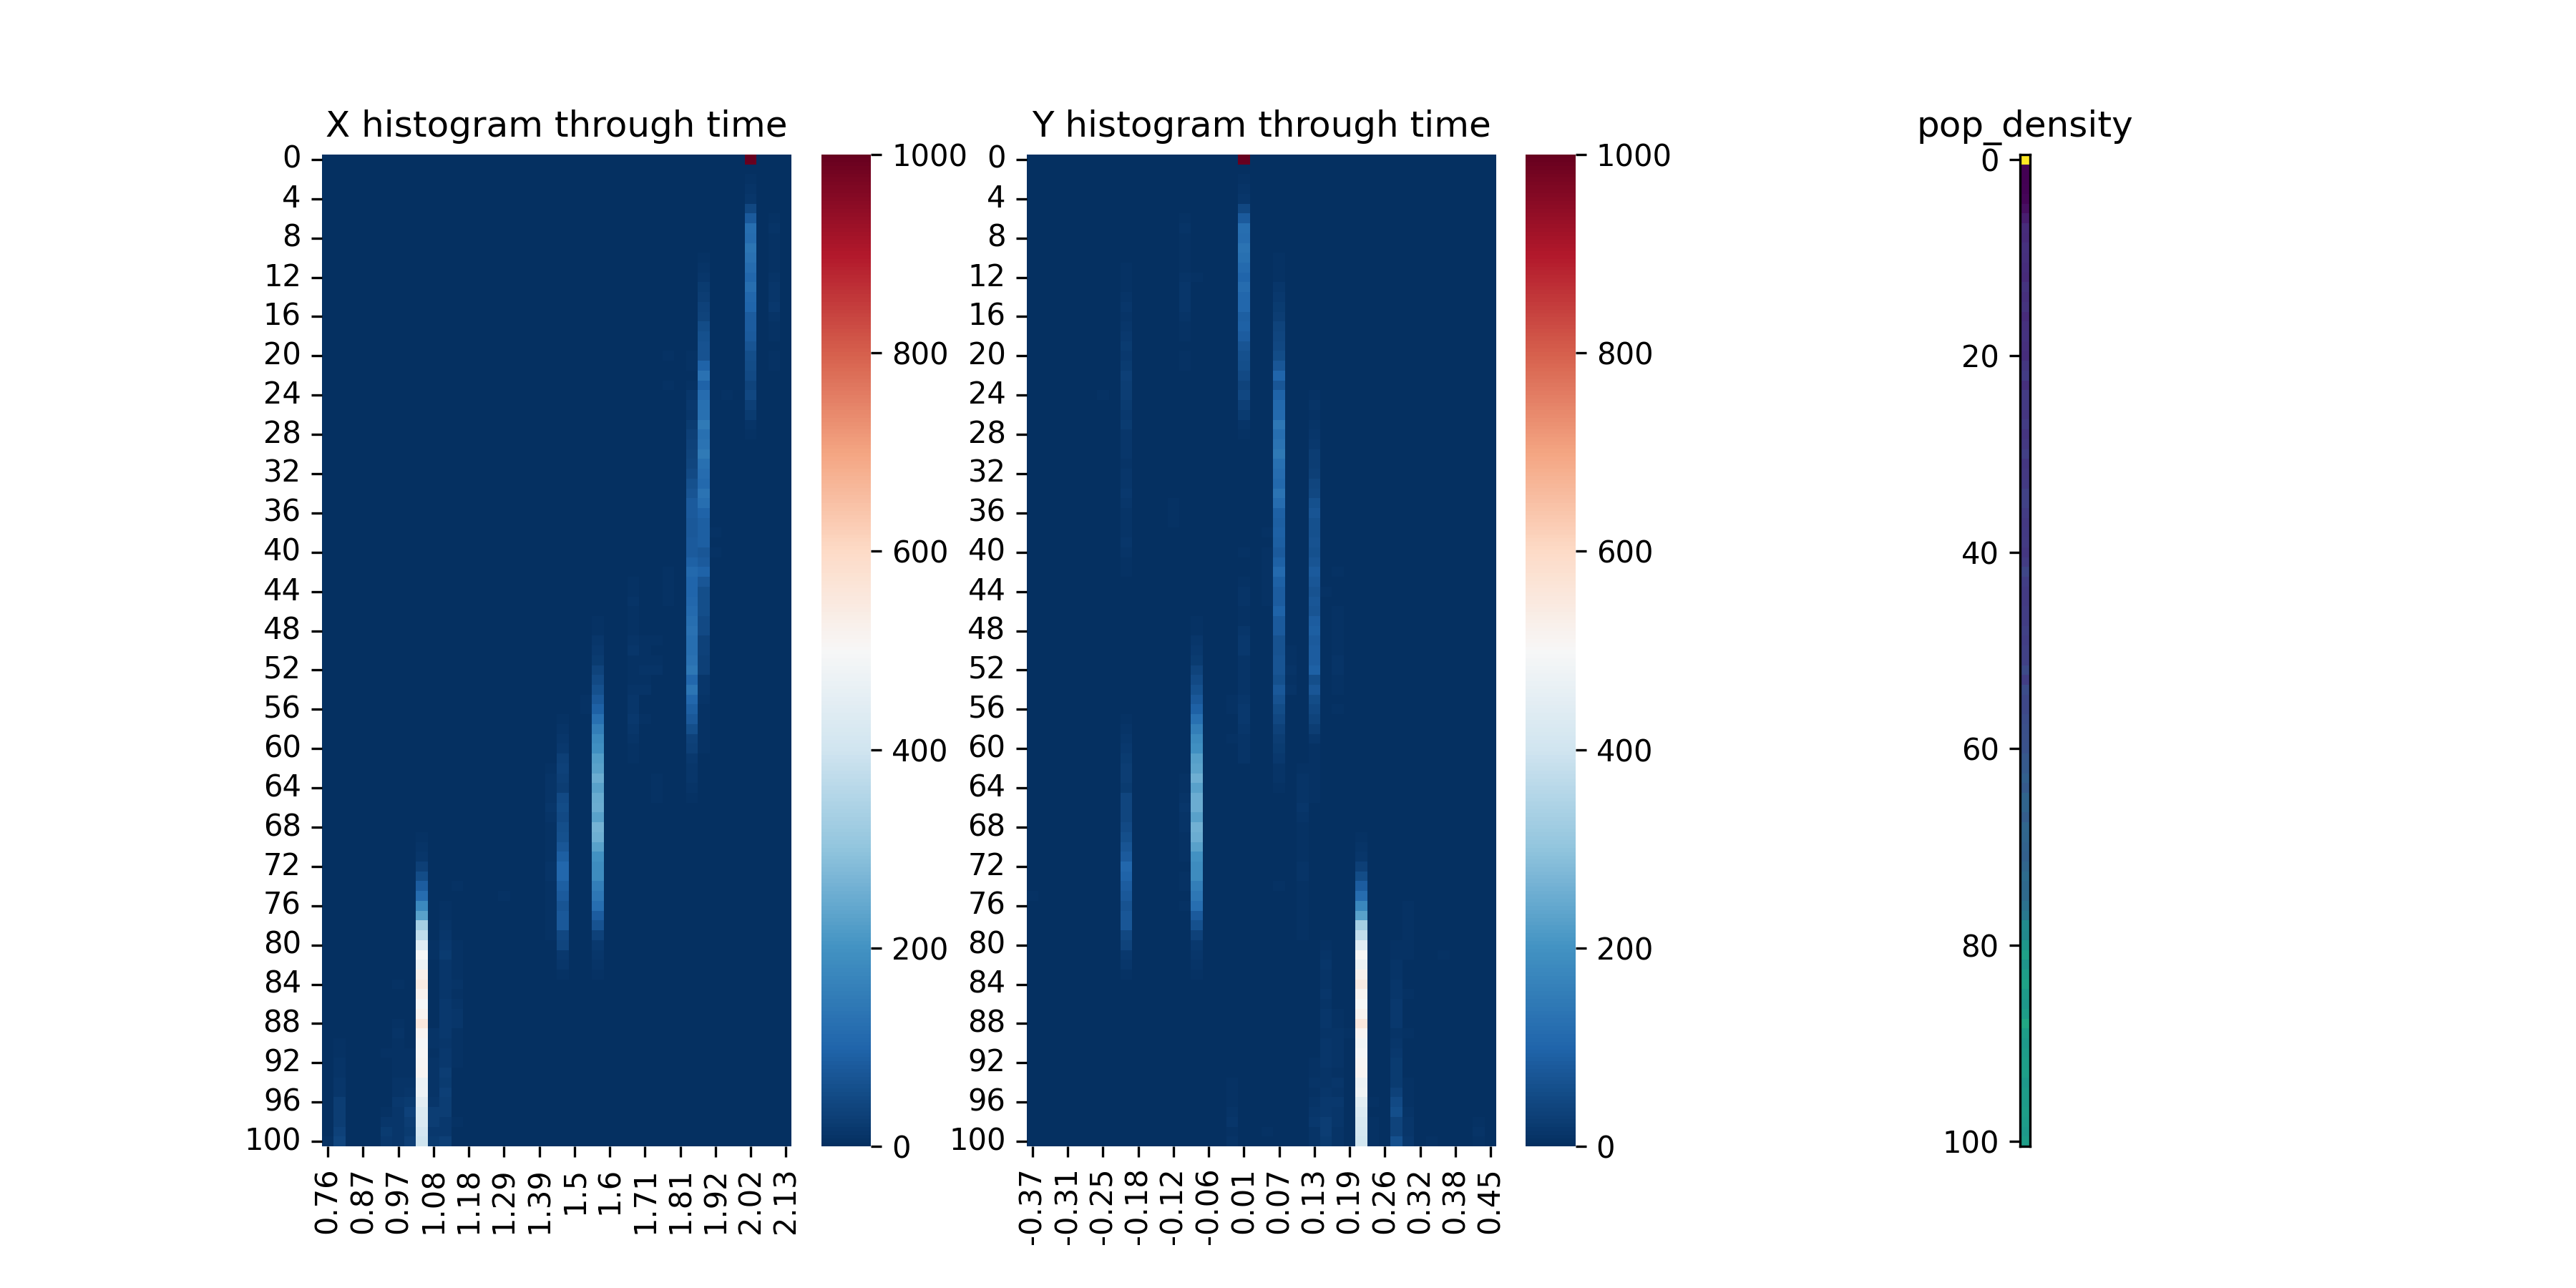
\includegraphics[scale=0.37]{x0_sc_sweep_(2.0)_(1)} \\
\textit{Heatmaps of $X$ and $Y$ for $\sigma_c=1$ and $x=1$ (top) and $x=2$ (bottom)}
\end{center}

Here, we see that when $x_0$ starts away from $x=0$, it "tries" to get back to $0$ because it's simultaneously trying to minimise competition with other individuals and maximise resource exploitation (with always happens at $x=0$). \\
As all individuals start at $x=0$, competition is really high, and the further $x_0$ starts from $x=0$, the lower $K(x_0)$ will be, then resulting in a higher and higher death rate, which explains why so many individuals don't proliferate in these graphs. \\
\vspace{5mm}


\subsubsection{$\sigma_k$ sweeps}

We can always set $\sigma_k = 1$ without loss of generality as it just changes the scale of $X$'s range. \\
However, we will be changing it to compare with all the other graphs for which $\sigma_k = 1$, to see just how much it changes this range. \\
\vspace{5mm}

\begin{center}
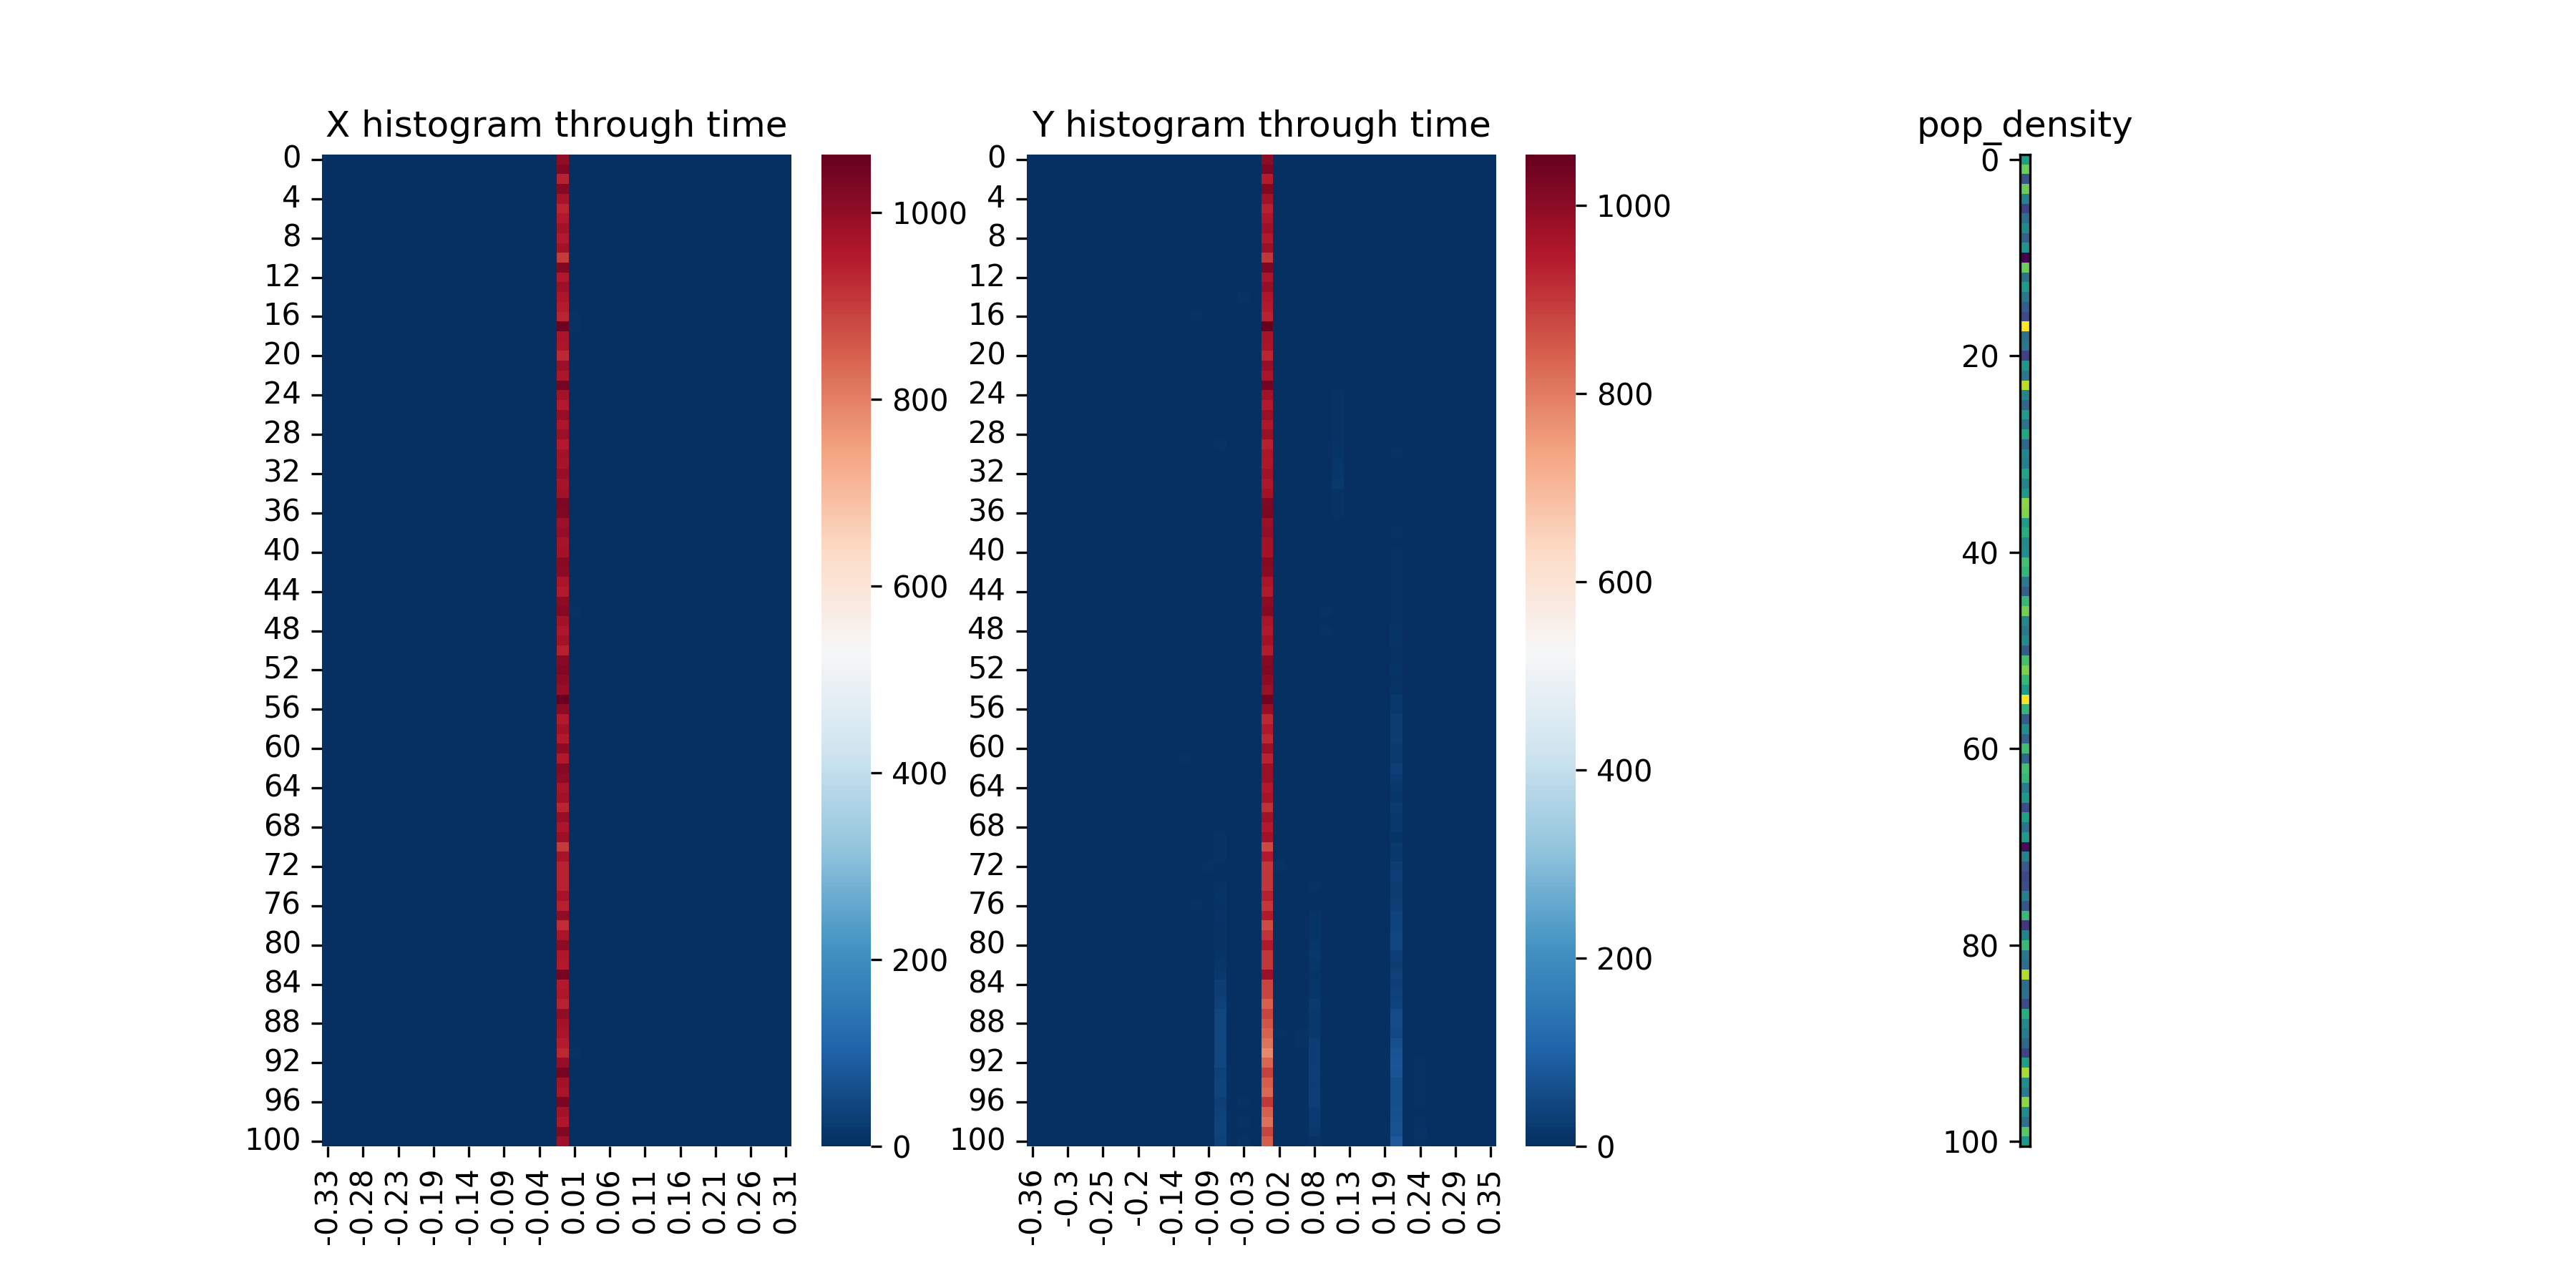
\includegraphics[scale=0.37]{x0_sk_sweep_(0.0)_(0.01)}
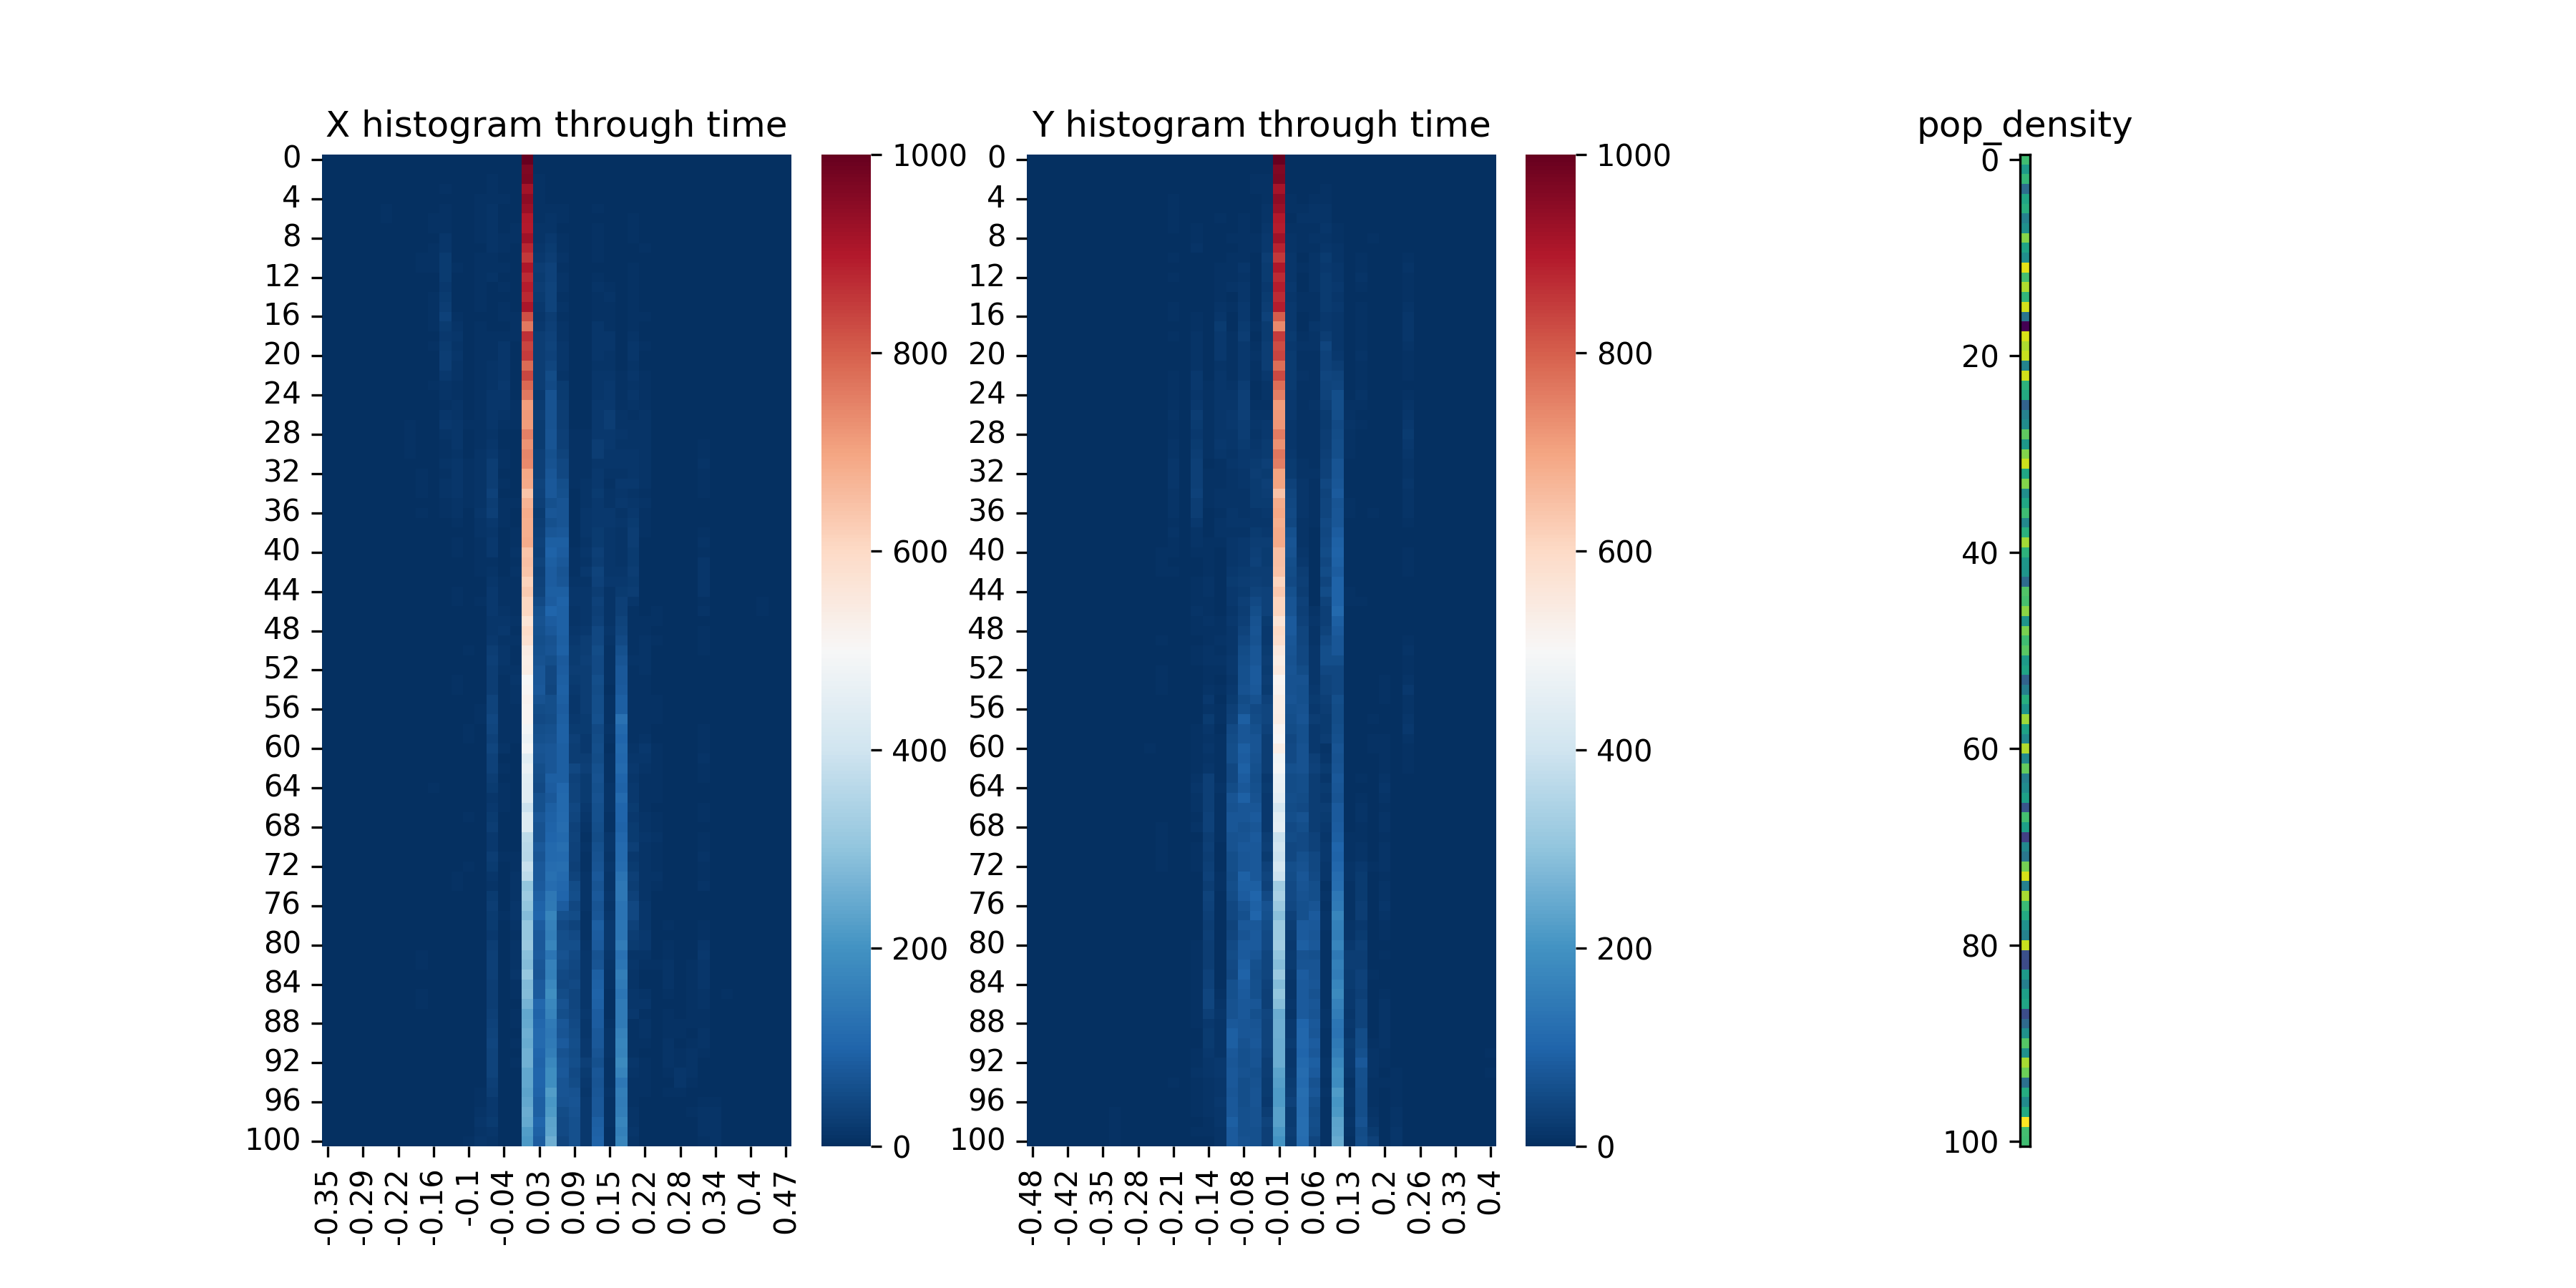
\includegraphics[scale=0.37]{x0_sk_sweep_(0.0)_(0.5)} \\
\textit{Heatmaps of $X$ and $Y$ for $x_0=0$ and $\sigma_k=0.01$ (top) and $\sigma_k=0.5$ (bottom)}
\end{center}

We can visualise the Gaussian curves representing relative competition $\alpha$ and resource exploitation $K(x)$ in a \textcolor{blue}{\underline{\href{https://www.geogebra.org/m/bzwgrcez}{graphing calculator}}} and clearly see that if $\sigma_k$ is too low, an optimal $x$ (when considering competition) tends to be really close to $0$. \\
When $\sigma_k$ is a little higher, the values of $x$ tend to be more evenly distributed, because as competition needs to be lower, it's better if individuals' $x$ values are further away from others'. \\
\vspace{5mm}

\begin{center}
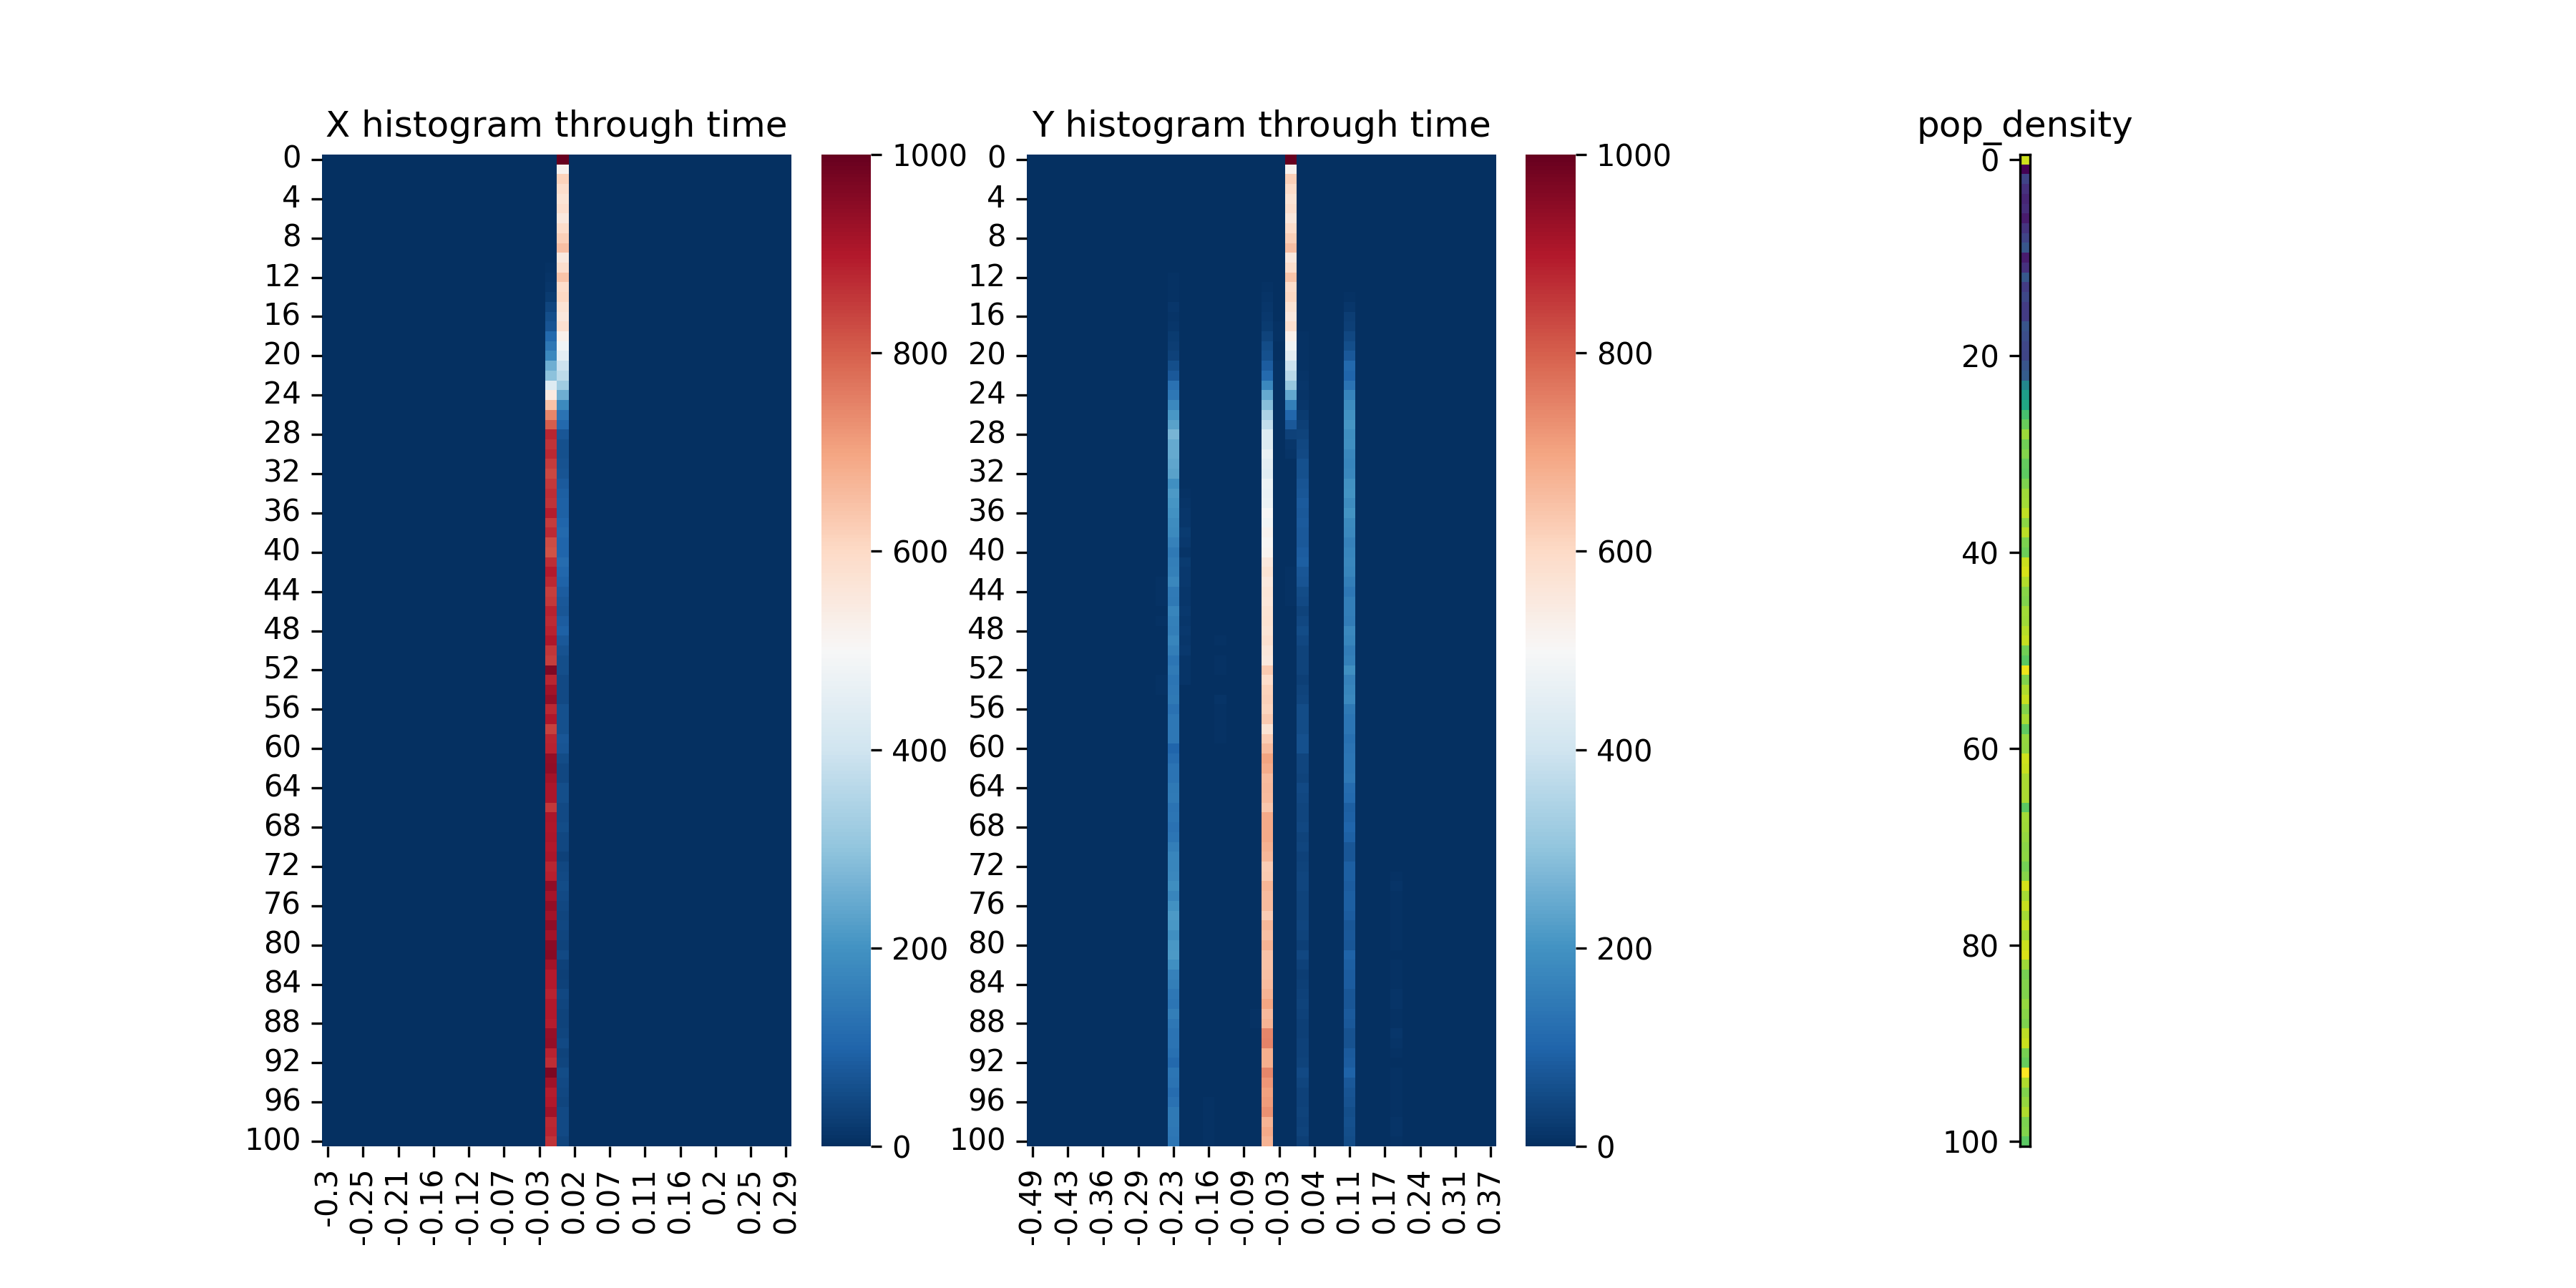
\includegraphics[scale=0.5]{x0_sk_sweep_(0.01)_(0.01).png}
\textit{Heatmaps of $X$ and $Y$ for $x_0=0.01$ and $\sigma_k=0.01$}
\end{center}

In this last graph, we can see that even if $x_0$ start really close to $0$, it's still not close enough considering how small the variance of $K$ is. \\
$x_0$ would need to be smaller for resource exploitation to be high enough to allow individuals to survive the extreme competitive environment of generation 0. \\
Because of this, we see half the population doesn't reproduce, and the other half gets to our stable point $x=0$. \\
\vspace{5mm}

This complete destruction of half the population is interesting : if this event were to happen all of a sudden in a population that was going through a transition due to an invasive allele for example, it could erase all traces of that allele and completely disrupt the transition. \\
\vspace{2mm}
This is, of course, purely situational, but it does raise the question of how relevant the model is if the only interesting aspect of the simulation, as far the $X$ trait is concerned, happens at the very first generation. \\
\vspace{5mm}

% Comments on results

% {r = 1, K0, sigma_k = 1000, 1, sigma_c = 1, n_bins = 40, beta = 0, mu, sigma_m = 0.01, 0.1}
% reading heatmap, X seems to strictly increase in time, while Y follows a more random-looking evolution, with clear mean displacement.
% looking at mean plots, it's clear that we could estimate a linear relationship between mean values of X and Y in time.

% Idea for later in the day :
% run simulation about 10 times and sweep over a parameter.




\section{Thoughts on the model}

The model claims to represent sympatric speciation with two evolving traits. \\
\vspace{5mm}

We were unable to find a subset of parameters that would allow for a bimodal distribution of either $X$ or $Y$. \\
\vspace{5mm}

The nature of $x$ values' influence on resource exploitation implies that fitness maximisation requires $\lvert x \rvert$ to be as small as possible and thence does not allow for bimodality. \\
\vspace{2mm}
Similarly, $y$'s only role in the model is to characterise a trait under directional selection. By definition, this almost necessarily prevents for a forking evolution as it will always yield a continuous movement following the direction given by $\beta$. \\
The fact that $\beta$ is not dynamic is the biggest offender here, as most uses of directional selection will include it as an adaptative form of selection (see equation $(5)$ from Nunney (2016), they implement directional selection to model movement towards current optimum \cite{Nun16}). \\
\vspace{5mm}

According to the population we want to model, we'd have to modify $\beta$ accordingly to properly represent how $Y$ values' optimum moves along with it. As the model stands, the optimum is always $\bar{Y}+\beta$, and can effectively be seen as $sgn(\beta) \infty$, with a cutoff  at $\lvert \beta \rvert$. \\
\vspace{1cm}

The main structure of the code written to generate all these graphs and run these simulations is stored \textcolor{blue}{\underline{\href{https://github.com/ChrisMzz/cmb-compbiol}{here}}}.



\bibliographystyle{alpha.bst}
\bibliography{compbiol_refs.bib}

\end{document}